\documentclass[11pt,letterpaper]{amsart}
\usepackage{anysize,fullpage,amssymb,latexsym,amsmath}
\marginsize{1in}{1in}{1in}{1in}%left,right,top,bottom%
\usepackage{graphicx}
\graphicspath{ {images/} }
\usepackage[mathscr]{eucal}
\usepackage{enumerate}
\usepackage{color}
\usepackage{hyperref}
\usepackage{float}
\usepackage{multirow}
\usepackage{amsmath}
\usepackage{comment}
\usepackage{listings}
\usepackage{ebgaramond}


\begin{document}
\begin{center}

\begin{LARGE}
\textbf{NBA Analysis}
\end{LARGE}\\
By Matias Sanchez\\
SFSU Fall 2022

\end{center}

\noindent \Large \textbf{Intro:} \leavevmode \newline\\

\indent Whenever the NBA or any sport is brought up, height/athleticism is mentioned as the key success factor. It is assumed that the taller a player is, the more effortless the game should be for them. Or if a player is shorter, it should be harder for them to perform well.\\

\indent The first part of the project aims to determine if the player’s physical aspects impact their play. There has also been an assumed correlation between a player’s height \& weight. The taller the person, the heavier they should be. That is no surprise. In the past, we have seen a change in taller or bigger NBA players on the court. There was a time when big players on a team dominated the game. However, the more modern NBA is dominated by guards or smaller players as the league evolved from post-dominant to shooting dominance.\\

\noindent Bigger and taller players had to get acclimated to today’s game. Thus, having a big player who can also score will require a semblance of shooting ability.\\

\noindent Although scoring tends to favor smaller players in the modern game, rebounding, an essential part of winning in the NBA, will be telling.  With fewer big players today, would rebounding favor smaller players who sneak in?\\ 

\noindent Also, how the big player is used in today’s game, in old school NBA, the big player would be essential in running an offense. Since smaller players now dominate it, would the big player be used as much as before?\\

\indent The second part we will be looking into is what contributes to winning. Many may say scoring is the most critical factor in winning a game, but scoring can merely tell one part of the story. Players may have a great scoring game, but they may win if the rest of the team is involved.\\

\noindent We will add a new data set to account for wins since it is not part of our other data. We will be using the variable of Win shares per 48 min, which has been accepted as how much a player contributed to the win in a 48 min span. This explains the variables most important in determining how much a player helps in the win.\\

\noindent There are also different types of win shares, offensive and defensive.  In analyzing this data, we may determine if it is more important to be better at defensive or offensive winning.
\\\\
\textbf{Chapter 1:}\\\\
\indent This chapter aims to determine if tall/big players are dying. We may determine that the taller the person, the less productive compared to smaller players. We will evaluate a player’s statistics through scoring, rebounding, true shooting percentage, and usage percentage. Points will be a specific player’s average score in that season. Rebounds will be the average rebounds for each player during that season. True shooting percentage is the player’s efficiency, considering free throws and two and 3-point field goals. Usage percentage is the percentage a player is used on offense while on the floor. The transition from a post-game to a shooting game will show how these teams choose to use their players and how the players have adapted to the game played today.\\
\cite{1} \leavevmode \newline\\
\noindent \textbf{{\large DATA:}} \\\\
\indent We will use linear regression, quantile regression, Poisson regression, and GAM to analyze the data.\\

\indent The data set we are using is taken from kaggle.com. The data set used consists of 11700 rows and 22 columns. The rows consist of each NBA player who played during 1996-97  and up to the 2020-21 season. Also, with the rows, there may be multiple players if they have played for numerous years in the NBA. The columns consist of 8 categorical variables and 14 numerical variables.
\\ \\
The variables that we focused on were:
\noindent
\begin{itemize}
\item \textbf{Player Height}: The height of that player for that season
\item \textbf{Points}: The average number of points per game for that player during that season
\item \textbf{Rebounds}: The average number of rebounds per game for that player during that season
\item \textbf{Usage percentage}: The percent that a player is used while on the floor during that season
\item \textbf{True shooting percentage}: The percent player shooting efficiency during that season
\end{itemize}
\cite{4}\\\\

\textbf{Chapter 2:}\\\\
\indent In chapter 2, we will also split the data into three separate eras. Splitting the eras could give us more information on how players have changed in different periods. Era one will consist of the span from 1997 to the 2004 season. Era 2 will be from 2005 to the 2013 season. Era 3 will be from 2014 to the 2022 season. This will better understand how the league has changed over time. Determine if helping your team win by performing in an area better in one era may hinder your team in a different period. Or it may just be an ” If it ain't broke, don't fix it” situation, and teams may not steer too far away from what has helped the past in winning. This section will separate the data into a training and test set to create an accurate prediction model. To find the best model we will, we will perform cross-validation. Cross-validation is when we separate the data into two segments; one is to train the model, and the other is to validate the model.\\

\noindent \textbf{{\large DATA:}} \\\\
\indent The data for this chapter was taken from basketball references. There needed to be a set of data to extract from. Thus, we had to create data tables by merging from separate forms to have the necessary variables for the second chapter.
\\ \\
The variables we focused on for chapter 2 were:\\
\noindent
\begin{itemize}
\item \textbf{PER (Player Efficiency Rating)}: The productivity of a player on a per-minute basis
\item \textbf{BPM (Box Plus/Minus)}: A box score estimate of points per 100 possessions a player contributed above league average
\item \textbf{WS/48 (Win shares per 48 Min)}: An estimate of the number of wins contributed by a player per 48 minutes
\end{itemize}
\cite{6}\\\\
\indent The analytical methods for Chapter 2 were Random Forest, Lasso Regression, and PCR.\\
\indent We will use the R program, a software environment for statistical computing and graphics, to evaluate the following methods with the data.
\\



\noindent \Large \textbf{Methods:}\\

\noindent \large \textbf{Method 1: Linear Regression}\\
\indent Linear regression is a simple method to produce a model to interpret easier. Linear regression models the relationship between x and a conditional mean dependent variable y. The linear regression model can be described as the following equation:

\begin{align*}
E(Y)&=\beta_0+\beta_1*x_1
\end{align*}
\\
\cite{5}\\
\indent The advantage of linear regression is that this model is easy to interpret. But if the model does not show a linear relationship, it will be inaccurate. If the dataset represents no linearity, it would be best to continue with quantile regression or other methods, as linear regression will not give an accurate result. However, we must check first to see if the two variables are fit to use the linear regression. The problem with using linear regression is that it assumes a linear relationship between the two variables, which is our assumption when using this method. Our assumptions for linear regression are that the y variable is normally distributed, there is a constant variable, and there is a linear relationship between the variables.\\
\indent A typical example we can use to fit linear regression is comparing the players’ height and weight. Since we expect the taller a person is, the heavier they will be. Thus, creating a linear property.
\\\\
\noindent \large \textbf{Method 2: Quantile Regression}\\
\indent Quantile regression will be the better option with our data as it is better used when there are many humps in our dependent variable. The model will be of the relationship between x and the conditional quantiles of y. Quantile regression is defined as the following equation:

\begin{align*}
Y_q&=\beta_0 + \beta_1x+\epsilon\\
y_i&=x_i'\beta_q+e_i
\end{align*}
\\
\textbf{$y_i$}= The response variable\\
\textbf{$x_i'$}= The derivative of the predictor variable\\
\textbf{$\beta_q$}= The vector of unknown parameters associated with the qth quantile.\\
\textbf{$e_i$}= The error of the response variable\\
\cite{2}\\
\indent As stated in linear regression, quantile regression can be used when data does not represent a linear relationship. This method is suitable since it could display different results for different predictor variables. It is also best used when the data has a comprehensive value Range, thus resulting in a non-linear relationship. Quantile regression does not make assumptions about the residual distribution and will help describe the distribution of the dependent variable. Since most of our data were unsuitable for linear regression, we will use quantile regression.
\\\\
\noindent \large \textbf{Method 3: Poisson Regression}\\
\indent Poisson will be used when the response variable is a count value. It will show how well the x variable is on the y variable. The Poisson regression model is similar to linear regression, except it will model the log of the expected value of y. The formula is as follows:

\begin{align*}
log(\lambda)=\beta_0+\beta_1x\\
\end{align*}
\\
\textbf{$\lambda$}= The expected response variable\\
\textbf{$\beta_0$}= The estimate of the intercept\\
\textbf{$\beta_1$}= The estimate of the predictor\\
\textbf{$x$}= The predictor variable\\
\cite{3}\\
\indent Poisson regression is best used when the response variable is count data. If our data has Over-dispersion, the data can cause the model to result in artificially minor standard errors leading to artificially small p-values for model coefficients. Some ways to counter dispersion are to use an estimated dispersion factor to inflate standard errors or use a negative binomial regression model.\\
\indent For Poisson regression, we looked more into a team-by-team basis. We decided which season was the best based on points and rebounds, then took all the teams for that season. For this evaluation, we will investigate the 2009 - 10 season. The results were only five significant teams for points, which resulted in a negative coefficient. Thus, this shows that the taller the person was for those five teams, the fewer points they would average for them. Other results from teams were significant in points but insignificant in rebounding. Although they depended on smaller players to score for them, they did not depend on height to get the rebounds. We also investigated one specific team throughout this period, resulting in the Los Angeles Lakers with exciting results.\\
\indent The results for the Lakers were mixed, some seasons depending on what players were on the team. This will be a common factor besides rebounding, points, and usage percentage, and true shooting percentage usually depends on what personnel is on the team.\\

\noindent \large \textbf{Method 4: GAM}\\
\indent We will use GAM. Since our model is nonlinear, we should get a better understanding. GAM’s flexibility and regularization should help get a better understandable solution. The model for GAM is as follows:
\begin{align*}
g(E(Y))= \alpha + s_1(x_1)
\end{align*}\\
\textbf{$Y$}= The response variable\\
\textbf{$x_1$}= The predictor variable\\
\textbf{$s_1$}= Smooth, nonparametric function\\
\textbf{$\alpha$}= The intercept coefficient\\
\textbf{$g(E(Y))$}= Link function, linking the expected value to the predictor variable\\
\cite{7} \leavevmode \newline
\indent GAM is good because it is easy to interpret, can uncover hidden patterns within the data and can help with overfitting. It is also great since it does not assume a linear relationship between the response and predictor. One drawback of using GAM is its predictability. Since GAM smoothing the variables, it may be out of range of the training dataset to make an accurate prediction. Although GAM is great for interpreting data, it may not be helpful when someone wants to use it for prediction.\\
\indent When deciding to use GAM, we decided to split the data into three different eras. GAM also showed an already-discovered pattern. When plotting GAM, it showed no relationship pattern between a player's performance and height. When comparing eras, we can deduce if there were any changes in how height impacted different performance stat.\\

\noindent \large \textbf{Method 5: Random Forest}\\
\indent Random Forest combines multiple decision trees to form a prediction on the y variable. This will work in this case since it is non-linear and will be used for mean prediction for regression. We will use it to find the most critical variables and as a prediction tool. This is an excellent tool since it will branch out multiple sections of the predictor variables and give a prediction. It will create various trees and then give the average based on the most critical variables.

\cite{8} \newline
\indent Random forest is helpful because it can be used for categorical and numerical data. Random forest is also not influenced by outliers in a dataset. Some drawbacks are the interpretations of the model. Random Forest will not give much on coefficients nor much control over how the model will run the data. Random Forest is an excellent tool for predicting and finding the most critical variables in the dataset. Still, if you want more information on how the data is functioning, it would be best to find a different method.\\

\noindent \large \textbf{Method 6: Lasso}\\
\indent Since our most essential variables from random forest had high correlation; we decided to use lasso while also separating the variables. The model of the lasso is to minimize the sum of squares by finding the best lambda to see the most shrinkage and accuracy. The model for Lasso is as follows: 
\begin{align*}
(\sum ^n_{i=1}(y_i - \sum_{j}x_{ij}\beta_j)^2 + \lambda \sum^p_{j=1} |\beta_j|
\end{align*}\\
\textbf{$y_i$}= Response variable\\
\textbf{$x_{ij}$}= The predictive variable\\
\textbf{$\beta_j$}= The estimate coefficients\\
\textbf{$\lambda$}= The amount of shrinkage being performed\\
\cite{9} \leavevmode \newline
\indent The good thing about Lasso is that it is a better tool for automatic variable selection than stepwise and forward and backward. The drawbacks are that it may ignore significant variables resulting in said significant variable being dropped. Another con of using lasso is that correlated variables may give different results. Like Random Forest, the lasso is limited in interpreting the dataset. It is great for variable selection and prediction, but other than that, it may be limited.\\
\indent Lasso is an accurate prediction method using shrinkage. Shrinkage is when the values of the data are shrunk towards a mean. This is great since there is no limit towards shrinkage. Lasso will shrink a variable to 0, determining how vital that variable is to the model.\\\\

\noindent \large \textbf{Method 7: PCR}\\
\indent Since our data has a high correlation in some variables, PCR became another option for prediction. PCR will find several principal components of linear combinations of the predictors. It will use least squares to fit a linear regression model while using the principle components. 
\begin{align*}
\beta_X = V\beta_Z
\end{align*}\\
\textbf{$\beta_X$}= Vector estimates of coefficients\\
\textbf{$V$}= Matrix of explanatory variables with eigenvectors as columns \\
\textbf{$\beta_Z$}= Vector estimates of coefficients based on matrix Z consisting of p principle components\\
\cite{10} \leavevmode \newline
\indent The advantages of PCR are that it can handle correlated data very well and handle overfitting in a dataset. As well as displaying results, this will work similarly to lasso, showing what variables are invalid and kicking them out. The disadvantage of PCR is that the data must be standardized to perform correctly. This can be tricky in prediction. If a training set is not standardized, then PCR might be biased toward high-variance features. Also, picking the number of components is essential. By selecting how many components to use, we can minimize the coefficients used in the model resulting in more accuracy. But, if the wrong number of components is selected, some information may be lost compared to its original list of features. As a result, PCR can still be effective for predicting a complex dataset, but it must be handled with caution to avoid errors.\\

\indent For the last section, we will compare Random Forest, Lasso, and PCR to find the best predictor model for determining a winner. Here we separated the data into three sections, Era 1, Era 2, and Era 3. Inside each era, we also looked at the total of the era and the top and bottom ten teams individually. We also had to normalize the data since some variables make the methods biased toward them.
\newpage \noindent \textbf{{\LARGE RESULTS}} \\\\

\begin{Large}
\textbf{Chapter 1: Height}
\end{Large}\\

\begin{center}
\emph{{\LARGE Method 1: Linear Regression}}
\end{center} \leavevmode \newline

%Describe model
\indent As stated in the methods section, linear regression was only usable in the relationship between height and weight. The relationship between height and any other variables exhibits non-linear tendencies. Thus, I will perform a comparison with a pair of variables that are valid and a pair that are not. As well as examining the assumptions of linear regression within them.
\begin{verbatim}
 ## 
## Call:
## lm(formula = nbau$player_weight ~ nbau$player_height)
## 
## Residuals:
##     Min      1Q  Median      3Q     Max 
## -27.397  -4.548  -0.169   4.215  41.104 
## 
## Coefficients:
##                      Estimate Std. Error t value Pr(>|t|)    
## (Intercept)        -1.265e+02  1.577e+00  -80.21   <2e-16 ***
## nbau$player_height  1.132e+00  7.886e-03  143.49   <2e-16 ***
## ---
## Signif. codes:  0 '***' 0.001 '**' 0.01 '*' 0.05 '.' 0.1 ' ' 1
## 
## Residual standard error: 6.98 on 9834 degrees of freedom
## Multiple R-squared:  0.6768, Adjusted R-squared:  0.6767 
## F-statistic: 2.059e+04 on 1 and 9834 DF,  p-value: < 2.2e-16
\end{verbatim} \leavevmode \newline

Linear regression was only useful when comparing height and weight. The output of this relationship is that height has a positive significance for weight, with the p-value being small. This indicates that the taller the player is, the heavier they will be, which is a given. As for why linear was not a good fit for the other variables, we have to see the plots.\\

\begin{figure}[H] 
%\vspace{-1.9cm}
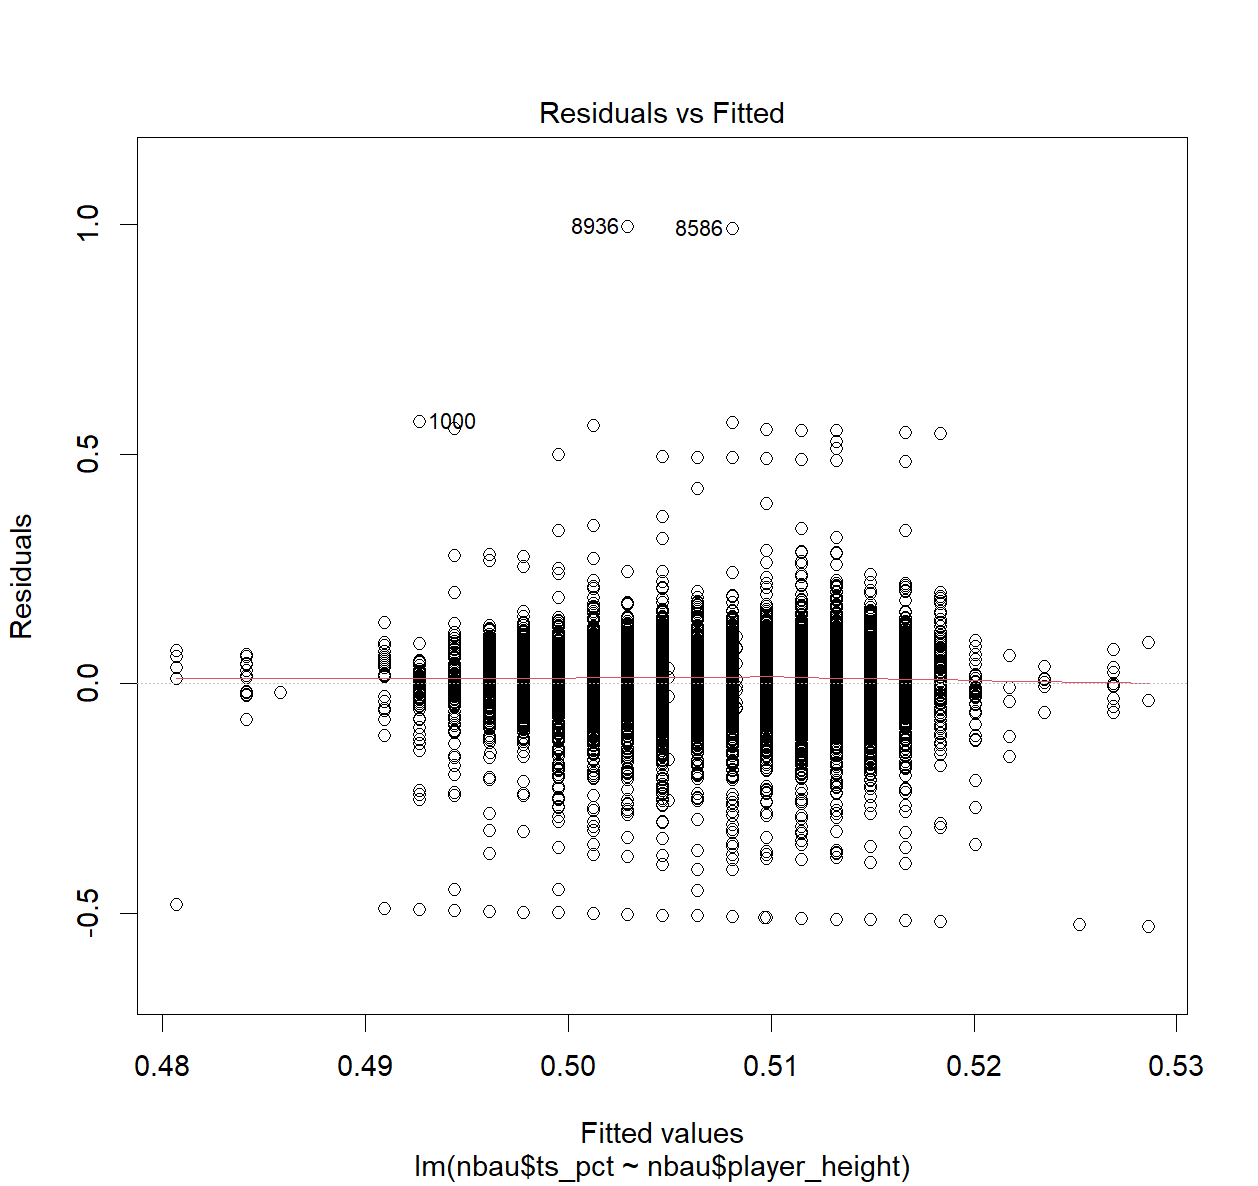
\includegraphics[width=0.4\textwidth]{lmplot1}\hspace{1cm}
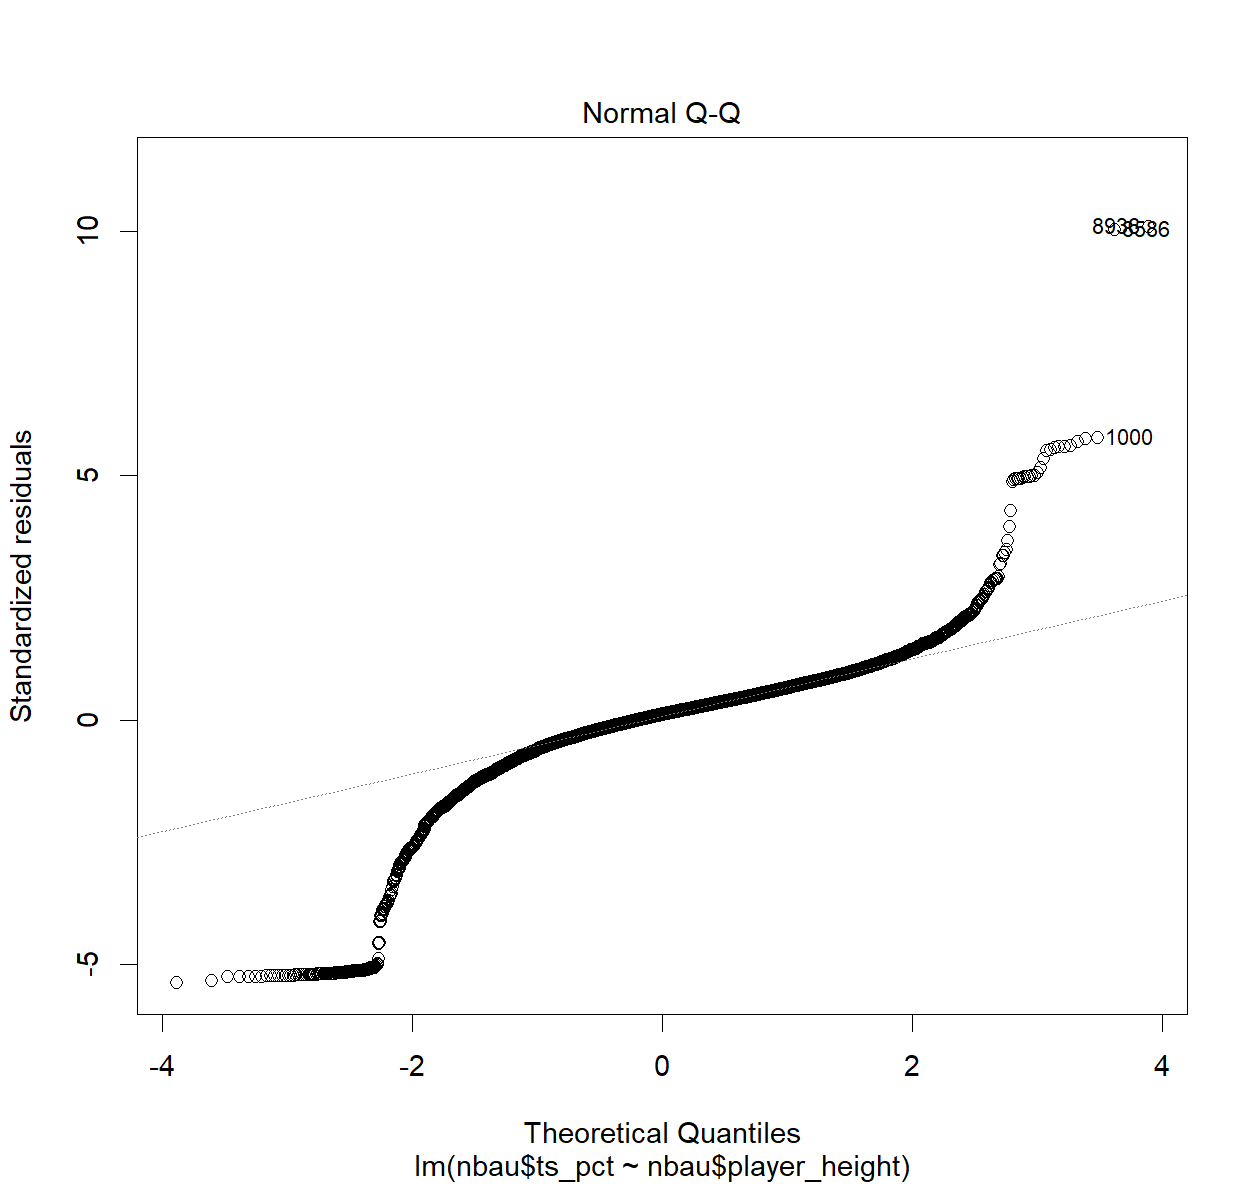
\includegraphics[width=0.4\textwidth]{lmplot2}\hspace{1cm}
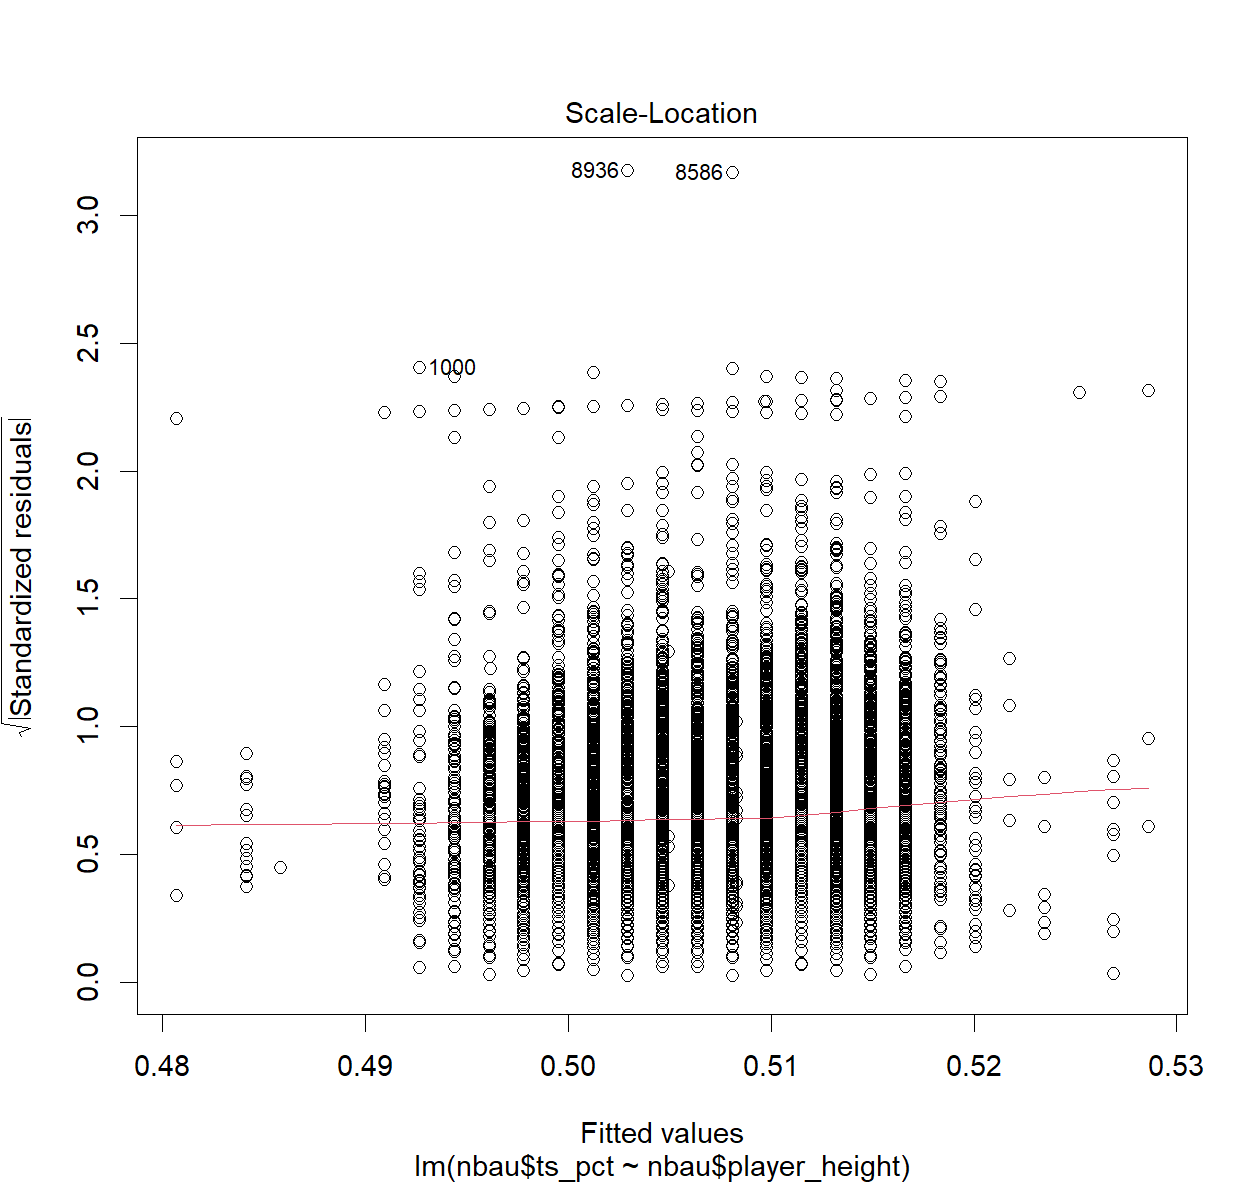
\includegraphics[width=0.4\textwidth]{lmplot3}\hspace{1cm}
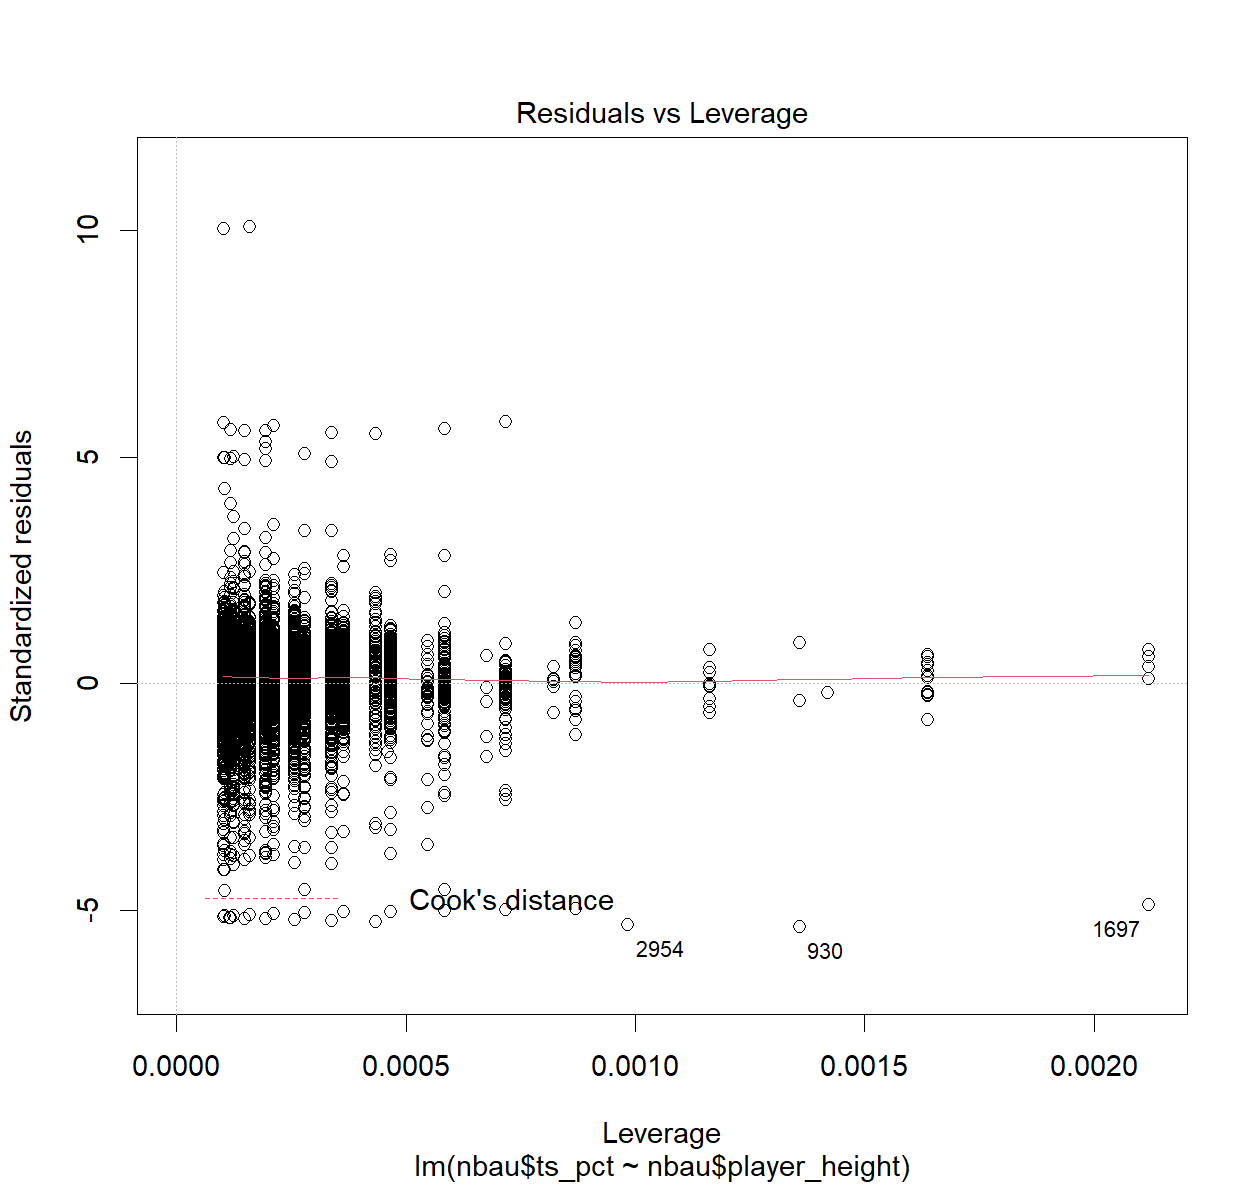
\includegraphics[width=0.4\textwidth]{lmplot4}\hspace{1cm}
\caption{The plots of TS percentage and Height linear regression. \label{fig1}}
\end{figure} \leavevmode 
\begin{figure}[H] 
%\vspace{-1.9cm}
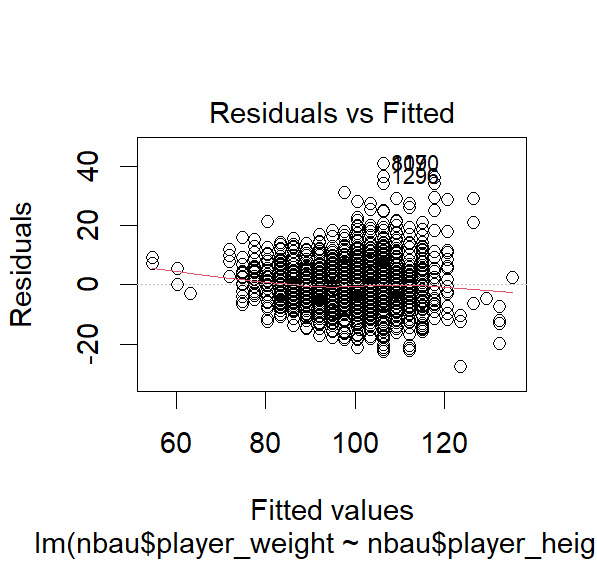
\includegraphics[width=0.4\textwidth]{lmplot5}\hspace{1cm}
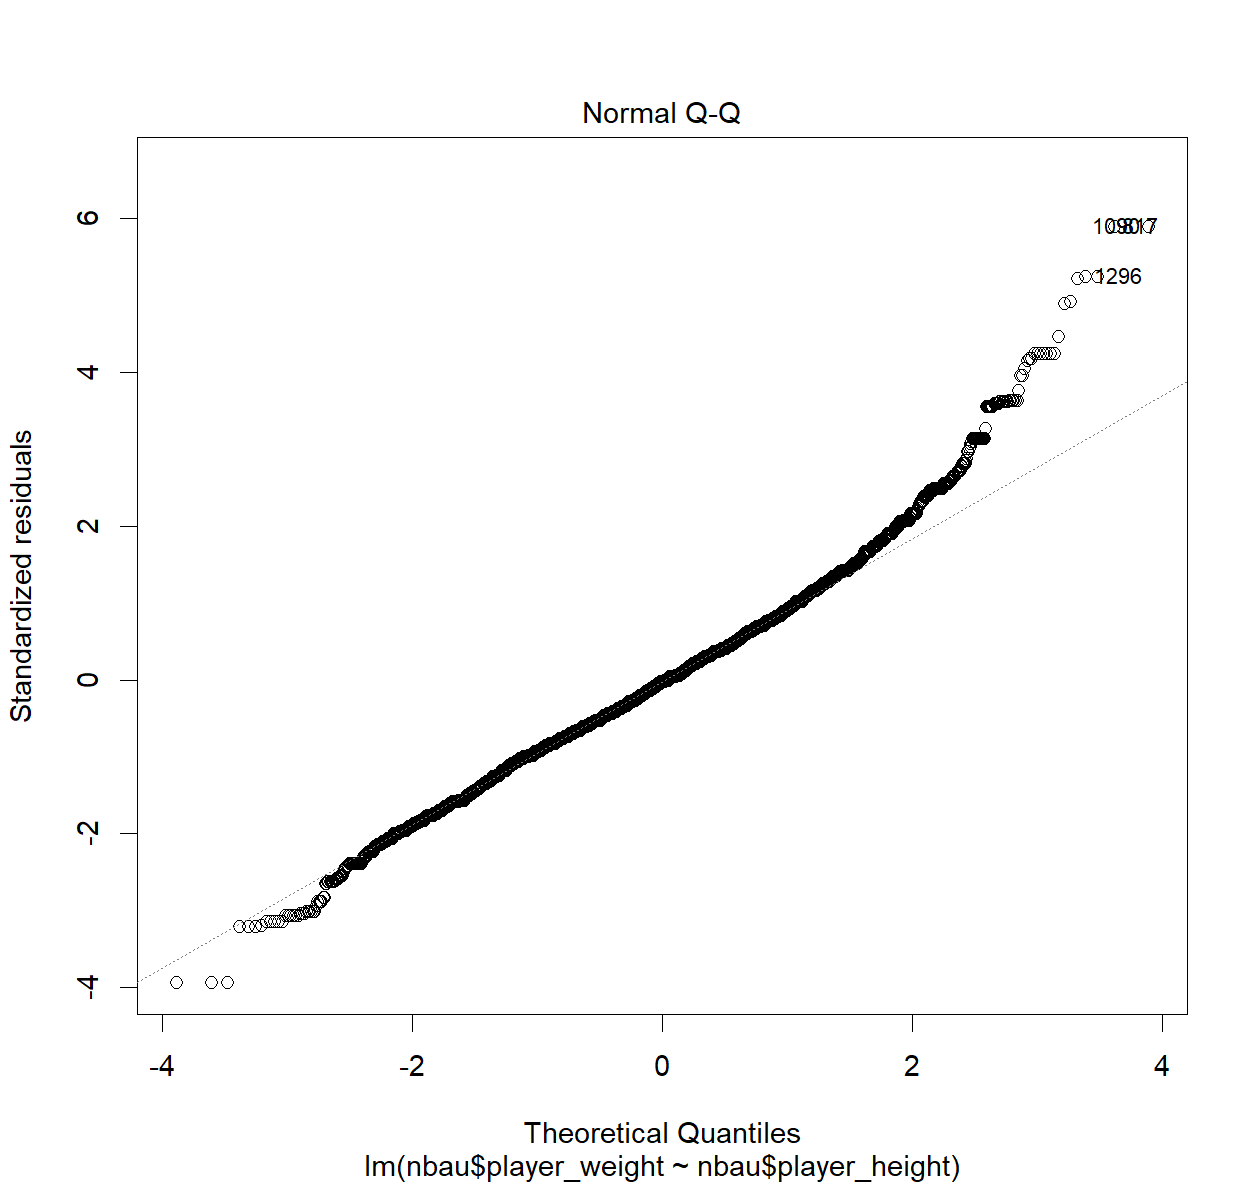
\includegraphics[width=0.4\textwidth]{lmplot6}\hspace{1cm}
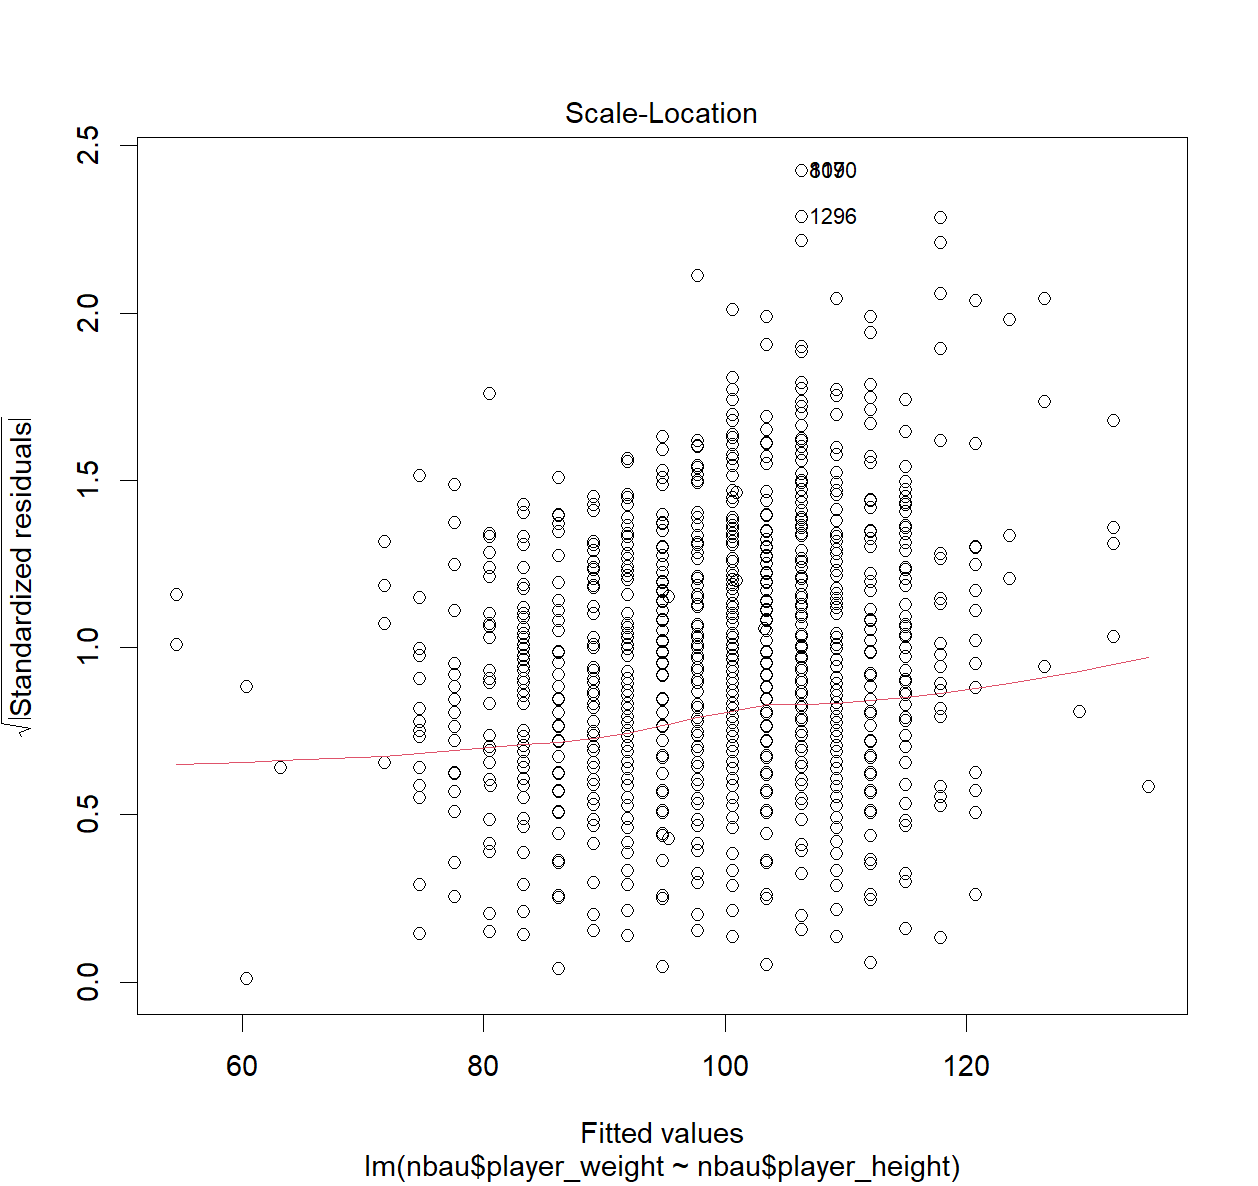
\includegraphics[width=0.4\textwidth]{lmplot7}\hspace{1cm}
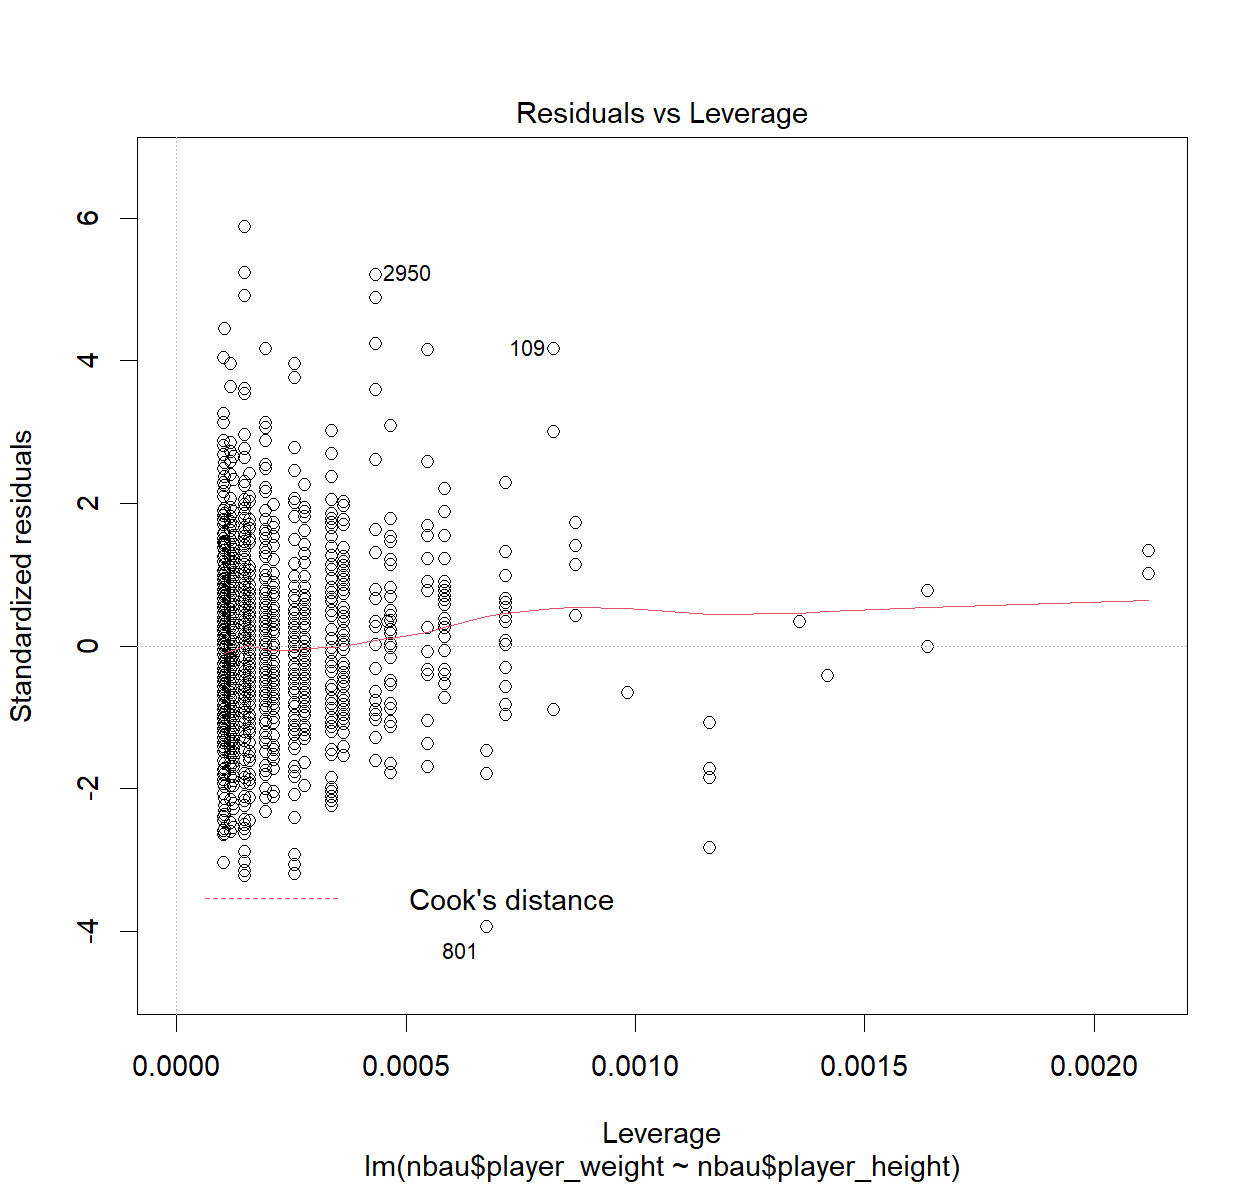
\includegraphics[width=0.4\textwidth]{lmplot8}\hspace{1cm}
%\vspace{-1.9cm}
\caption{The plots of Weight and Height linear regression. \label{fig2}}
\end{figure} \leavevmode
Figure 1 shows the relationship between Height and true shooting percentage. Figure 2 shows the plots for the relationship between Weight and Height. In both figures, the top left image is the residual vs fitted plot. This will show if there is a linear relationship. In order to arrive at a linear relationship, there should be no distinctive pattern. As we can see, there is no pattern in height and TS percentage compared to the weight plot. The height and weight plot show no pattern at all. Therefore, Ts percentage does not pass the linear relationship assumption, but height and weight do. Next, we will look at the normal Q-Q plots. Normal Q-Q plots will show whether the residuals are normally distributed. As we can see from the TS percentage and height plot, the residuals are not normally distributed. In the plot, the dots dramatically stray off the red line at the ends. It would be best if the dots were close to the red line. However, it does stray a bit at the ends of the height and weight plot, but not enough to warrant abnormality. Thus we can confidently say that height and weight do not violate linear regression assumptions. In comparison, height and any other variables used in this chapter failed the assumptions of linear regression. These failed assumptions are present in all combinations of height and non-weight variables.\\
\\
\newpage
\begin{center}
\emph{{\LARGE Method 2: Quantile Regression}}
\end{center} \leavevmode \newline

%Tell story\\
\indent When our relationships failed the assumptions of linear regression, we would run them through quantile regression. Unlike linear regression, quantile regression does not consider assumptions about the data. Also, linear regression uses least squares to calculate the conditional mean, while quantile regression estimates the conditional median. There is a greater sense of control over the process of analyzing the data that we are given.\\
\begin{verbatim}
## 
## Call: rq(formula = nbau$ts_pct ~ nbau$player_height, tau = 0.9)
## 
## tau: [1] 0.9
## 
## Coefficients:
##                    Value    Std. Error t value  Pr(>|t|)
## (Intercept)         0.35500  0.02306   15.39750  0.00000
## nbau$player_height  0.00118  0.00012   10.10377  0.00000
\end{verbatim}


\begin{verbatim}
## 
## Call: rq(formula = nbau$usg_pct ~ nbau$player_height, tau = 0.9)
## 
## tau: [1] 0.9
## 
## Coefficients:
##                    Value    Std. Error t value  Pr(>|t|)
## (Intercept)         0.30857  0.02212   13.95126  0.00000
## nbau$player_height -0.00028  0.00011   -2.50965  0.01210
\end{verbatim}\leavevmode \newline
\indent The USA results were that the true shooting percentage was significant, at the 90 percent Quantile, and with a positive coefficient. Thus, we can say that for a player from the USA, the taller they are, the better the true shooting percentage they will have.\\
\indent As for usage percentage, also 90 percent quantile, the USA player’s height was significant but had a negative coefficient. For a player from the USA, the taller they were, they were used less on offense by teams.\\\\
\indent We also investigated merging the players. Instead of having multiple seasons for the player, all the seasons for that player were combined to create one row for each player. This data will look at the true shooting percentage and usage percentage when the players are merged. \\
\begin{verbatim}
## 
## Call: rq(formula = nba.players$ts_pct ~ nba.players$player_height, 
##     tau = 0.95)
## 
## tau: [1] 0.95
## 
## Coefficients:
##                           Value   Std. Error t value Pr(>|t|)
## (Intercept)               0.34307 0.03712    9.24276 0.00000 
## nba.players$player_height 0.00127 0.00020    6.48051 0.00000
\end{verbatim}\leavevmode \newline
\indent The results for true shooting were at 95 percent quantile, as it was significant with a positive coefficient. Thus, on average, throughout a player's NBA career, the taller the player, the better the true shooting percentage that player will have.

\begin{verbatim}
## 
## Call: rq(formula = nba.players$usg_pct ~ nba.players$player_height, 
##     tau = 0.3)
## 
## tau: [1] 0.3
## 
## Coefficients:
##                           Value    Std. Error t value  Pr(>|t|)
## (Intercept)                0.36540  0.02604   14.03292  0.00000
## nba.players$player_height -0.00102  0.00013   -7.91330  0.00000
\end{verbatim} \leavevmode \newline
\indent As for usage percentage, at 30 percent quantile, it was significant but with a negative coefficient. Thus, in this instance, the taller the person, the less they will be used by the team.\\
\newpage
\begin{center}
\emph{{\LARGE Method 3: Poisson Regression}}
\end{center} \leavevmode \newline

\indent Now we will concentrate on count data by using poisson. The poisson model is similar to linear regression, except it takes the log of the expected Y variable. This section is also the first time we've focused on certain teams. The teams we will be looking at are all the teams separated throughout the data. We will focus on one team, the Los Angeles Lakers, throughout all its years. The variables we will be analyzing are points and rebounds. We would assume that rebounds should be in favor of taller players, but there were instances where they were not. \\
\begin{verbatim}
## 
## Call:
## glm(formula = nba.season10GSW$pts ~ nba.season10GSW$player_height, 
##     family = "poisson")
## 
## Deviance Residuals: 
##     Min       1Q   Median       3Q      Max  
## -2.9663  -0.8643  -0.3696   1.1109   2.1427  
## 
## Coefficients:
##                               Estimate Std. Error z value Pr(>|z|)    
## (Intercept)                   11.45691    1.91367   5.987 2.14e-09 ***
## nba.season10GSW$player_height -0.04540    0.00964  -4.710 2.48e-06 ***
## ---
## Signif. codes:  0 '***' 0.001 '**' 0.01 '*' 0.05 '.' 0.1 ' ' 1
## 
## (Dispersion parameter for poisson family taken to be 1)
## 
##     Null deviance: 54.825  on 16  degrees of freedom
## Residual deviance: 31.885  on 15  degrees of freedom
## AIC: Inf
## 
## Number of Fisher Scoring iterations: 4
\end{verbatim}

\begin{verbatim}
## 
## Call:
## glm(formula = nba.season10GSW$reb ~ nba.season10GSW$player_height, 
##     family = "poisson")
## 
## Deviance Residuals: 
##     Min       1Q   Median       3Q      Max  
## -1.0588  -0.5619  -0.1095   0.3786   1.1740  
## 
## Coefficients:
##                               Estimate Std. Error z value Pr(>|z|)
## (Intercept)                   -1.32356    3.01119  -0.440    0.660
## nba.season10GSW$player_height  0.01388    0.01490   0.932    0.352
## 
## (Dispersion parameter for poisson family taken to be 1)
## 
##     Null deviance: 8.5789  on 16  degrees of freedom
## Residual deviance: 7.7056  on 15  degrees of freedom
## AIC: Inf
## 
## Number of Fisher Scoring iterations: 4
\end{verbatim}




\begin{verbatim}
## 
## Call:
## glm(formula = nba.season10POR$reb ~ nba.season10POR$player_height, 
##     family = "poisson")
## 
## Deviance Residuals: 
##     Min       1Q   Median       3Q      Max  
## -1.2063  -0.8122  -0.1388   0.1537   1.6033  
## 
## Coefficients:
##                                Estimate Std. Error z value Pr(>|z|)    
## (Intercept)                   -13.33724    3.23745  -4.120 3.79e-05 ***
## nba.season10POR$player_height   0.07257    0.01565   4.638 3.51e-06 ***
## ---
## Signif. codes:  0 '***' 0.001 '**' 0.01 '*' 0.05 '.' 0.1 ' ' 1
## 
## (Dispersion parameter for poisson family taken to be 1)
## 
##     Null deviance: 35.7621  on 14  degrees of freedom
## Residual deviance:  9.7898  on 13  degrees of freedom
## AIC: Inf
## 
## Number of Fisher Scoring iterations: 5
\end{verbatim}

\begin{verbatim}
## 
## Call:
## glm(formula = nba.season10POR$pts ~ nba.season10POR$player_height, 
##     family = "poisson")
## 
## Deviance Residuals: 
##     Min       1Q   Median       3Q      Max  
## -3.1491  -1.8888  -0.0610   0.4643   3.8220  
## 
## Coefficients:
##                               Estimate Std. Error z value Pr(>|z|)
## (Intercept)                   0.156831   1.826136   0.086    0.932
## nba.season10POR$player_height 0.009875   0.009039   1.092    0.275
## 
## (Dispersion parameter for poisson family taken to be 1)
## 
##     Null deviance: 55.893  on 14  degrees of freedom
## Residual deviance: 54.683  on 13  degrees of freedom
## AIC: Inf
## 
## Number of Fisher Scoring iterations: 5
\end{verbatim}\leavevmode \newline
\indent The results, for points, were that only five teams out of 30 were significant. All five of those teams that were significant resulted in a negative coefficient. Thus, this shows that the taller the person was for those five teams, the less they would average for them. Above is the result from one of the teams that were significant in points but insignificant in rebounding. Although they depended on smaller players to score for them, they did not depend on height to get the rebounds.\\
\indent The results for rebounds were mixed. Only 16 teams had a significance in rebounding depending on height, which surprised us. Usually, a team would want taller players to get easier rebounds, but in the case of 14 teams, the size was not significant in their rebounding. Of those 16 teams, all had a positive coefficient. Thus, the taller the person for those teams, the more rebounds they would get. Above are the results for the Portland team. They resulted in significance in rebounding but insignificant in points. Thus, they relied on the big players to get rebounds but not so much on scoring.\\\\
\indent For our second evaluation, we looked at all the seasons for one team. The best team we picked was the Los Angeles Lakers, and we will be looking at points and rebounds for this team.\\

\begin{verbatim}
## 
## Call:
## glm(formula = nba.LAL16$pts ~ nba.LAL16$player_height, family = "poisson")
## 
## Deviance Residuals: 
##     Min       1Q   Median       3Q      Max  
## -2.5265  -0.9766  -0.3338   0.8798   2.5002  
## 
## Coefficients:
##                         Estimate Std. Error z value Pr(>|z|)    
## (Intercept)              9.80917    2.18398   4.491 7.08e-06 ***
## nba.LAL16$player_height -0.03837    0.01094  -3.506 0.000454 ***
## ---
## Signif. codes:  0 '***' 0.001 '**' 0.01 '*' 0.05 '.' 0.1 ' ' 1
## 
## (Dispersion parameter for poisson family taken to be 1)
## 
##     Null deviance: 39.219  on 14  degrees of freedom
## Residual deviance: 26.831  on 13  degrees of freedom
## AIC: Inf
## 
## Number of Fisher Scoring iterations: 4
\end{verbatim}


\begin{verbatim}
## 
## Call:
## glm(formula = nba.LAL16$reb ~ nba.LAL16$player_height, family = "poisson")
## 
## Deviance Residuals: 
##      Min        1Q    Median        3Q       Max  
## -1.05231  -0.64506  -0.03416   0.20124   2.56371  
## 
## Coefficients:
##                         Estimate Std. Error z value Pr(>|z|)
## (Intercept)             -3.24583    3.27111  -0.992    0.321
## nba.LAL16$player_height  0.02256    0.01606   1.405    0.160
## 
## (Dispersion parameter for poisson family taken to be 1)
## 
##     Null deviance: 12.765  on 14  degrees of freedom
## Residual deviance: 10.786  on 13  degrees of freedom
## AIC: Inf
## 
## Number of Fisher Scoring iterations: 4
\end{verbatim}

The results for points were fascinating. The lakers had nine seasons out of 25, which was significant. This is interesting because, between 98 and 03, the lakers had a dominant big player who could score in Shaquille O’Neal. Thus, it would make sense that we had significance with a positive coefficient between those years. But then Shaq left the team, and there were three separate occasions between the years 2004 to 2021 when the lakers had significance. Those three significant years also had a positive coefficient, except for one year. That one year also resulted in an insignificant in rebounds. Thus, we can say that in 2016, the big players for the lakers were not good. They were negligible in rebounding and were not outputting a lot in scoring.\\




\begin{verbatim}
## 
## Call:
## glm(formula = nba.LAL04$reb ~ nba.LAL04$player_height, family = "poisson")
## 
## Deviance Residuals: 
##     Min       1Q   Median       3Q      Max  
## -1.2360  -0.8325  -0.4034   0.6670   1.6550  
## 
## Coefficients:
##                          Estimate Std. Error z value Pr(>|z|)    
## (Intercept)             -11.22819    3.84860  -2.917 0.003529 ** 
## nba.LAL04$player_height   0.06208    0.01874   3.313 0.000923 ***
## ---
## Signif. codes:  0 '***' 0.001 '**' 0.01 '*' 0.05 '.' 0.1 ' ' 1
## 
## (Dispersion parameter for poisson family taken to be 1)
## 
##     Null deviance: 24.304  on 14  degrees of freedom
## Residual deviance: 12.700  on 13  degrees of freedom
## AIC: Inf
## 
## Number of Fisher Scoring iterations: 4
\end{verbatim}


\begin{verbatim}
## 
## Call:
## glm(formula = nba.LAL04$pts ~ nba.LAL04$player_height, family = "poisson")
## 
## Deviance Residuals: 
##     Min       1Q   Median       3Q      Max  
## -2.5201  -1.7454  -0.6295   0.6827   4.4978  
## 
## Coefficients:
##                         Estimate Std. Error z value Pr(>|z|)
## (Intercept)             0.184512   2.479346   0.074    0.941
## nba.LAL04$player_height 0.009644   0.012224   0.789    0.430
## 
## (Dispersion parameter for poisson family taken to be 1)
## 
##     Null deviance: 67.923  on 14  degrees of freedom
## Residual deviance: 67.296  on 13  degrees of freedom
## AIC: Inf
## 
## Number of Fisher Scoring iterations: 5
\end{verbatim} \leavevmode
\indent As for rebounds, the Lakers had 21 out of 25 significant seasons. This is not at all surprising because most teams heavily rely on tall players to grab rebounds. The Lakers are one of those teams. All 21 of the significant seasons resulted in a positive coefficient. Thus, for most of the laker season, if they had a tall player, that player would be responsible for most of their rebounds. According to basket reference, the 2004 season was the last season Shaquille O’Neal played for the lakers. In his final year, Shaq’s output in points dropped by 6 points. Shaq averaged 27.5 points the previous year, while in 2004, he averaged 21.5. But his rebounding stayed the same. Therefore, the lakers had significance in rebounding but not in points for tall players. Another player, most likely a smaller player, had high output in scoring.\\
\cite{6}\\

\newpage
\begin{center}
\emph{{\LARGE Method 4: GAM}}
\end{center} \leavevmode\\
\indent In this section, we will evaluate the dynamics of the data. We will separate the data into three sections, or eras. The goal will be to determine whether having a certain height benefits a player statistically over a certain period of time. With this method, we can see whether height affects whether a player achieves a statistical advantage or not. The GAM method will provide a visual representation of how a variable changes with our non-linear data.
\begin{figure}[H] 
%\vspace{-1.9cm}
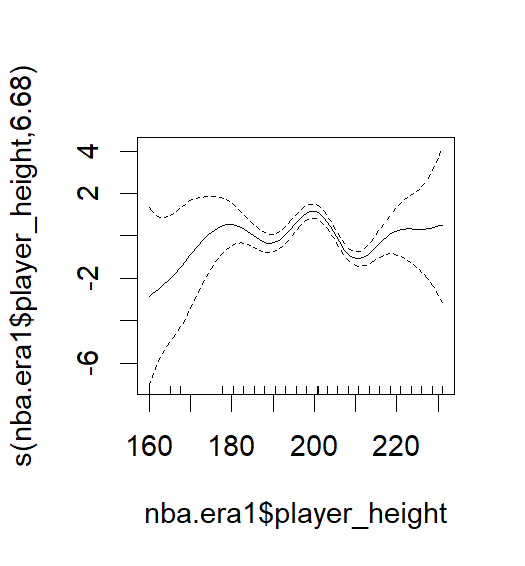
\includegraphics[width=0.4\textwidth]{Era1PTS}\hspace{1cm}
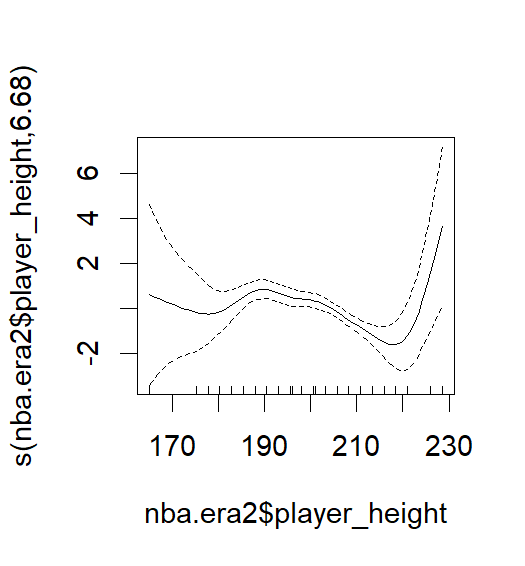
\includegraphics[width=0.4\textwidth]{Era2PTS}\hspace{1cm}
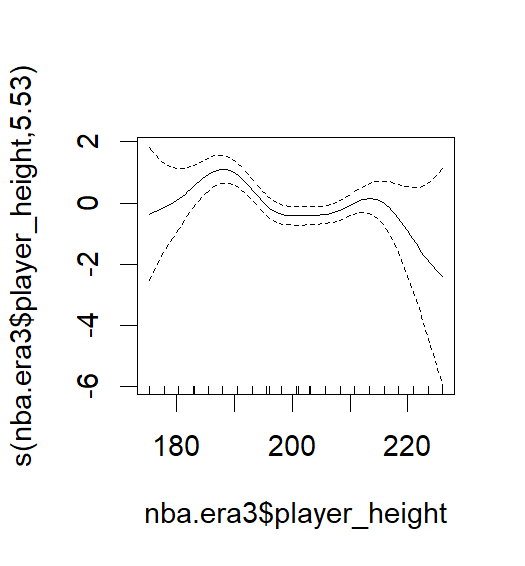
\includegraphics[width=0.4\textwidth]{Era3PTS}\hspace{1cm}
%\vspace{-1.9cm}
\caption{The three eras using GAM to analyze the relationship between Height and Points. \label{fig3}}
\end{figure} \leavevmode

\indent As we can see, the pattern between the three eras is that there is no pattern. In era 1, points were more effective by players in mid-height. As for era 2, shorter and taller players were more affected. In era 3, even smaller players were affected more, with a dip in the middle players. This shows the need for a pattern in determining the height effect. We can see that it varies by era. Thus, it shows that height does not affect the number of points a player scores. Height is merely an attribute for a player. No matter how tall or short a player is, they will only score as much if they have the skill to achieve.\\\\
\indent Next, we will see the relationship between height and a player’s true shooting percentage. We would assume that the taller the player is, the better percentage they would have. Since the taller player would be closer to the basket; thus, it should be easier to convert on opportunities.

\begin{figure}[H] 
%\vspace{-1.9cm}
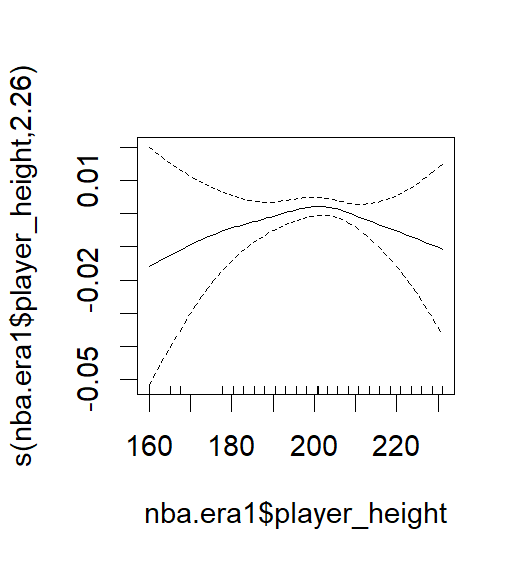
\includegraphics[width=0.4\textwidth]{Era1ts}\hspace{1cm}
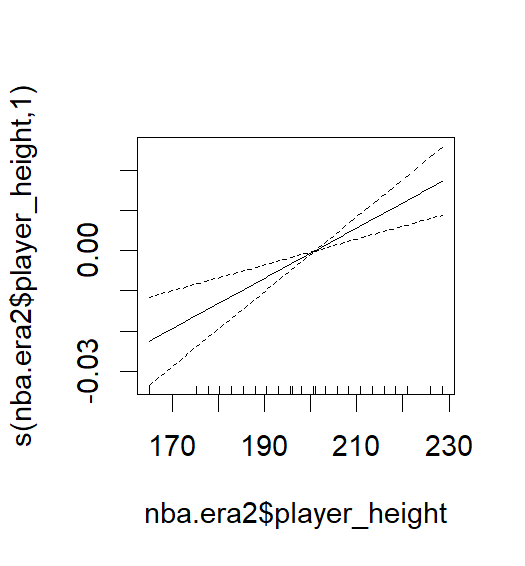
\includegraphics[width=0.4\textwidth]{Era2ts}\hspace{1cm}
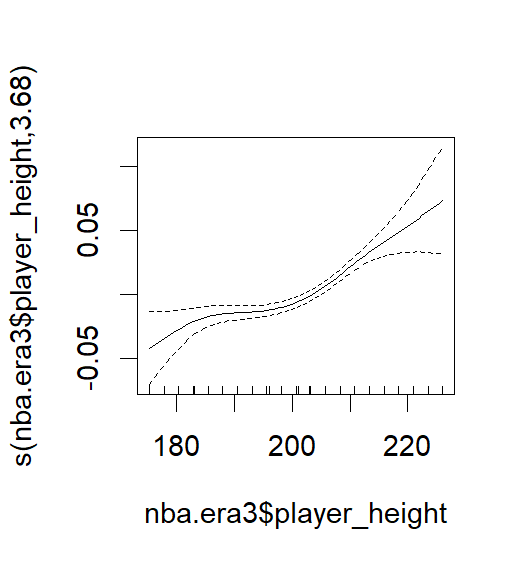
\includegraphics[width=0.4\textwidth]{Era3ts}\hspace{1cm}
%\vspace{-1.9cm}
\caption{The three eras use GAM to analyze the relationship between Height and True shooting percentage. \label{fig4}}
\end{figure} \leavevmode

\indent As we can see in the three figures, there is no discernible pattern. This is like the points figures when a different height is most affected in each era. This shows that a specific size does not give a player a better true shooting percentage.\\\\
\indent Finally, we will look at the relationship between height and usage percentage. In the early eras, there would be dominated by prominent big players in terms of usage. Then there would be a pull toward smaller players.

\begin{figure}[H] 
%\vspace{-1.9cm}
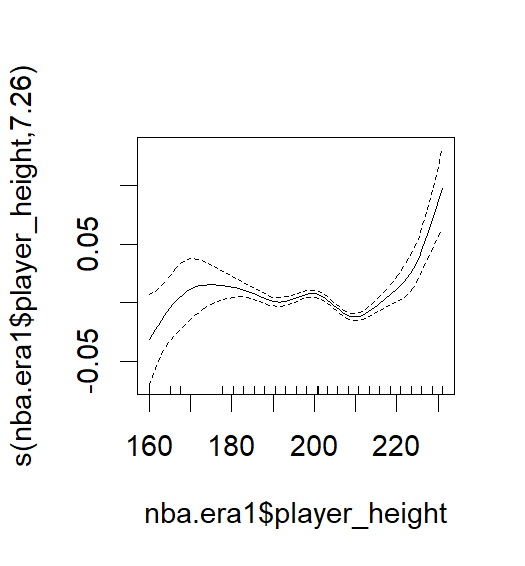
\includegraphics[width=0.4\textwidth]{Era1us}\hspace{1cm}
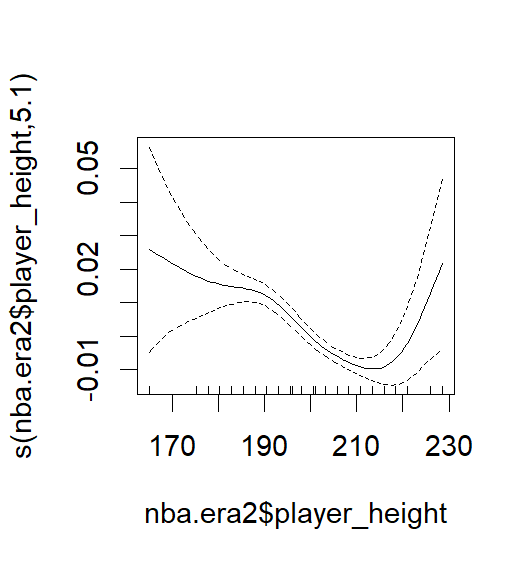
\includegraphics[width=0.4\textwidth]{Era2us}\hspace{1cm}
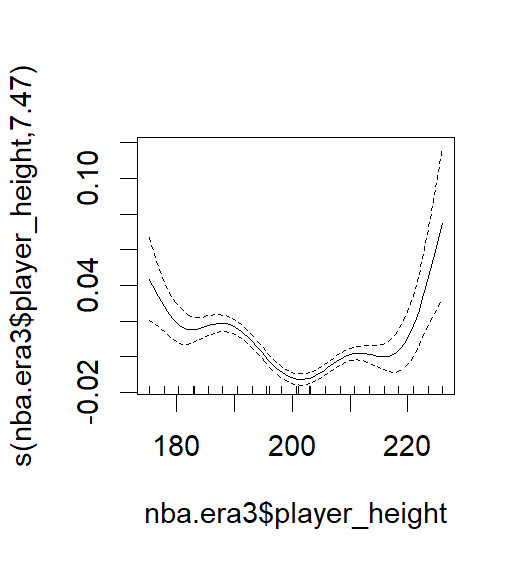
\includegraphics[width=0.4\textwidth]{Era3us}\hspace{1cm}
%\vspace{-1.9cm}
\caption{The three eras use GAM to analyze the relationship between Height and Usage percentage. \label{fig5}}
\end{figure} \leavevmode

\indent Here, we can see some consistency, especially with taller players. In each era, the tallest players and the most effective. At the same time, the smaller and medium players fluctuated between eras. This does not dispute how the other relationships have gone. Although the tallest is consistent, the smaller players are not. Thus, a player’s height cannot predict how well they will be in usage percentage.\\
\indent In the end, GAM showed no patterns or consistency between each relationship. This indicates that a player’s height cannot be a predictor alone to determine how well a player is.\\\\

\newpage
\begin{Large}
\textbf{Chapter 2: Win Shares}
\end{Large}\\

\begin{center}
\emph{{\LARGE Methods: Random Forest/Lasso Regression/PCR}}
\end{center} \leavevmode\\
\indent Lastly, we will examine what variables lead to winning. This will be interesting because many assume that the more points a player scores, the more they contribute. However, on the contrary, it is more complex. We will also look at what models best predict how much a player contributes to winning. We will include some advanced stats commonly used around the NBA to evaluate players. Height will not be a focus in this chapter. This is mainly because we have concluded that height does not affect a player's performance in the previous chapter. Thus, we will only focus on one variable, Win shares per 48 minutes, while including every other variable in the three different models. The three models we will be using are Random Forest, Lasso, and PCR.
\begin{figure}[H] 
%\vspace{-1.9cm}
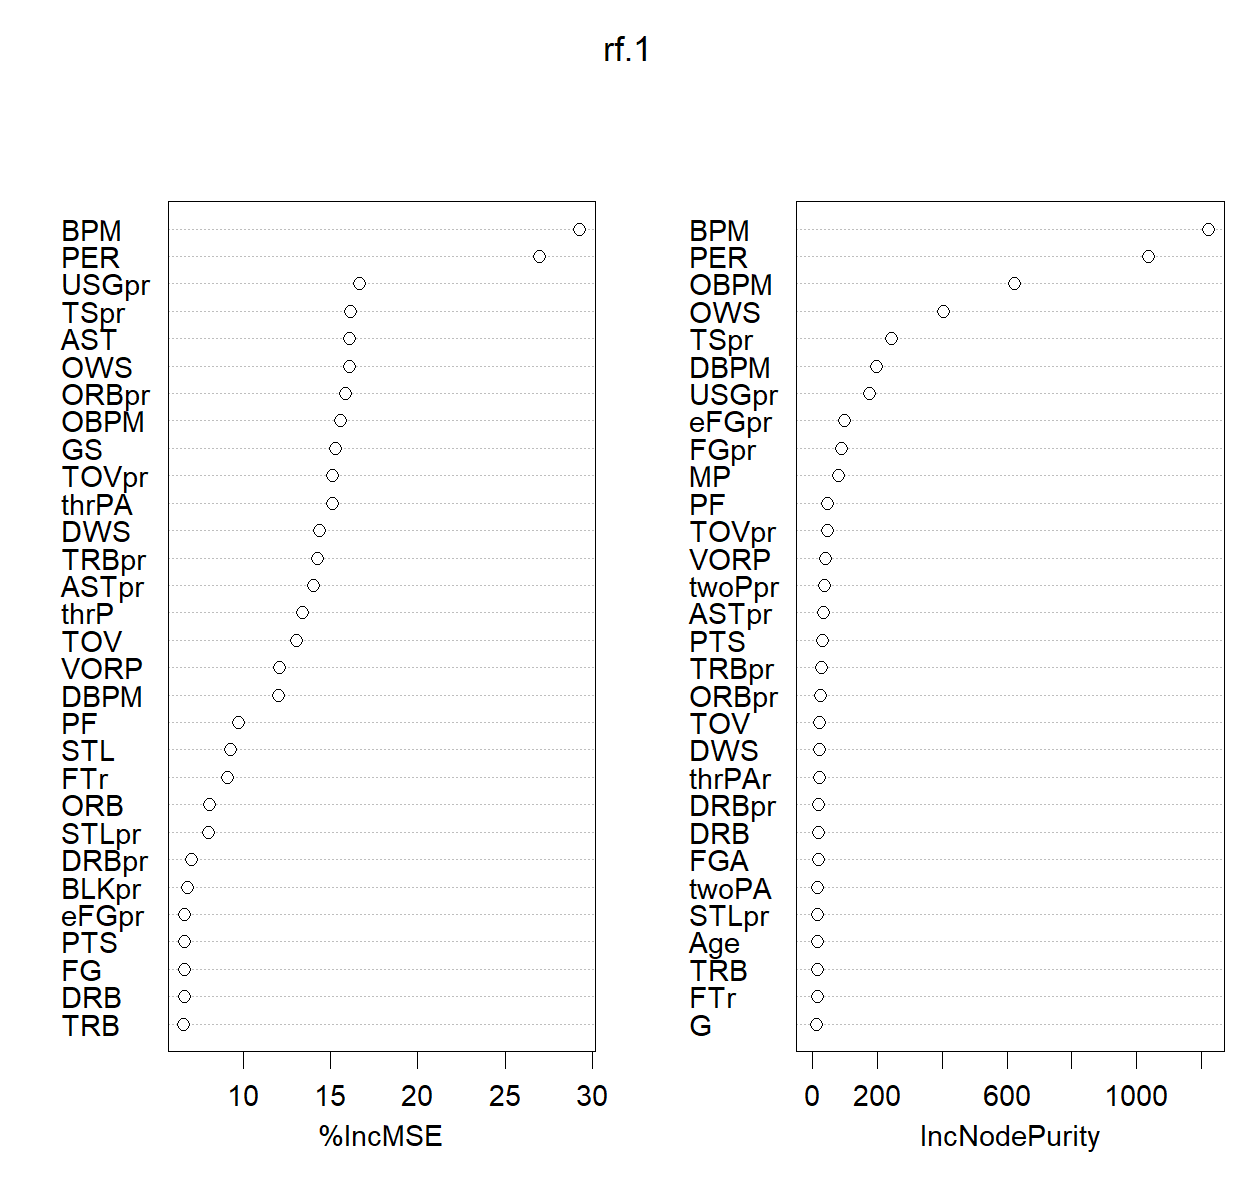
\includegraphics[width=0.4\textwidth]{rfera1}\hspace{1cm}
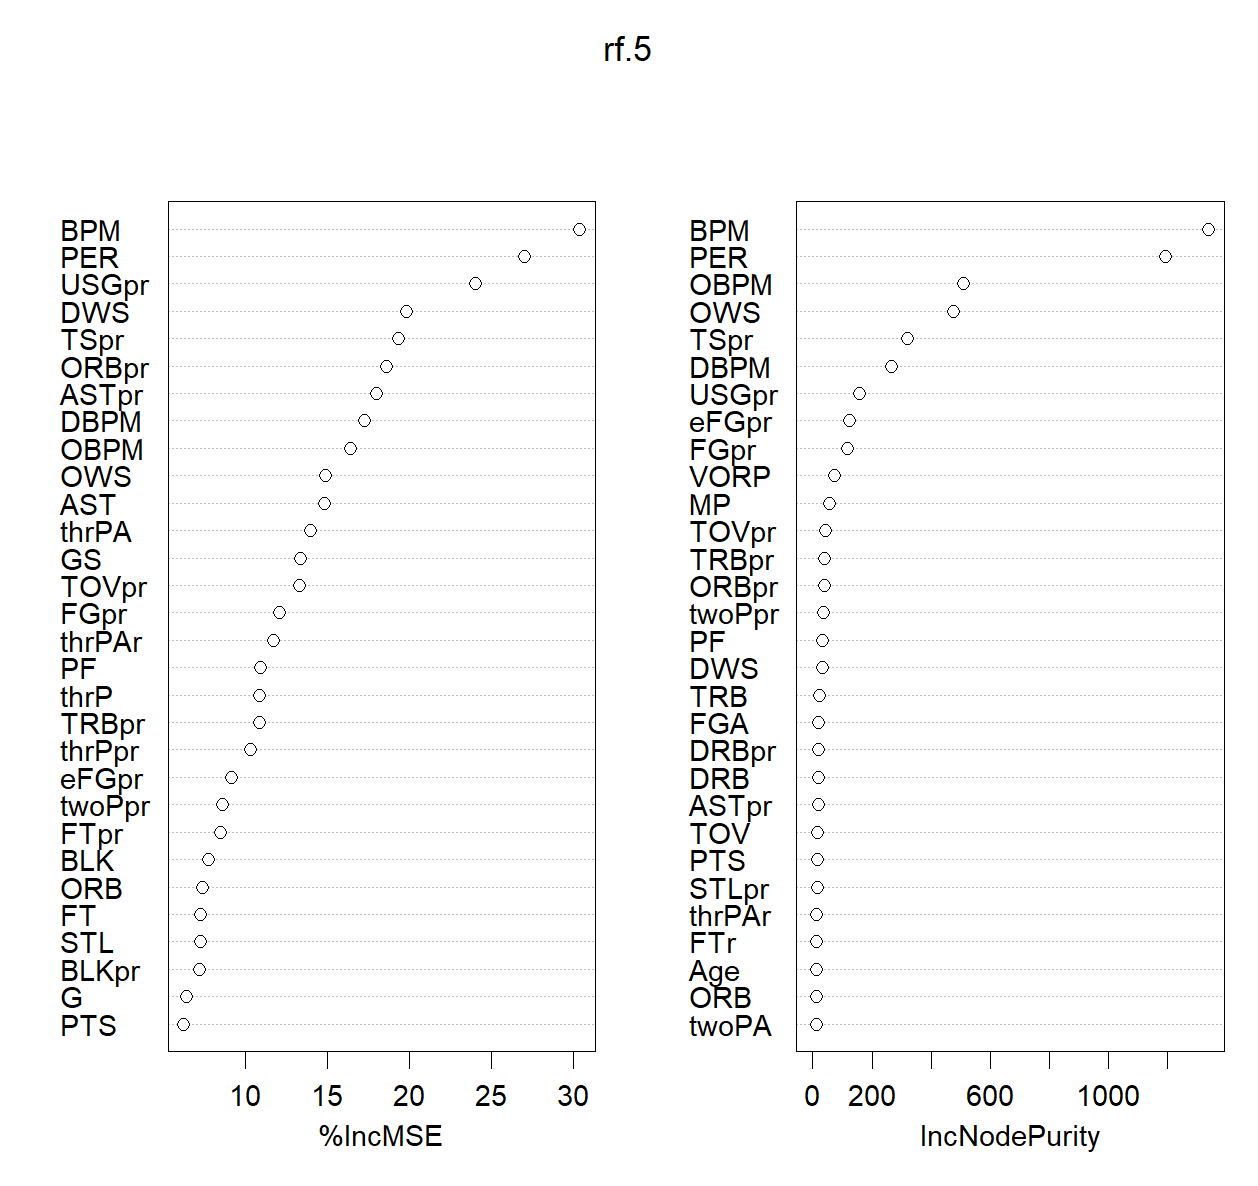
\includegraphics[width=0.4\textwidth]{rfera2}\hspace{1cm}
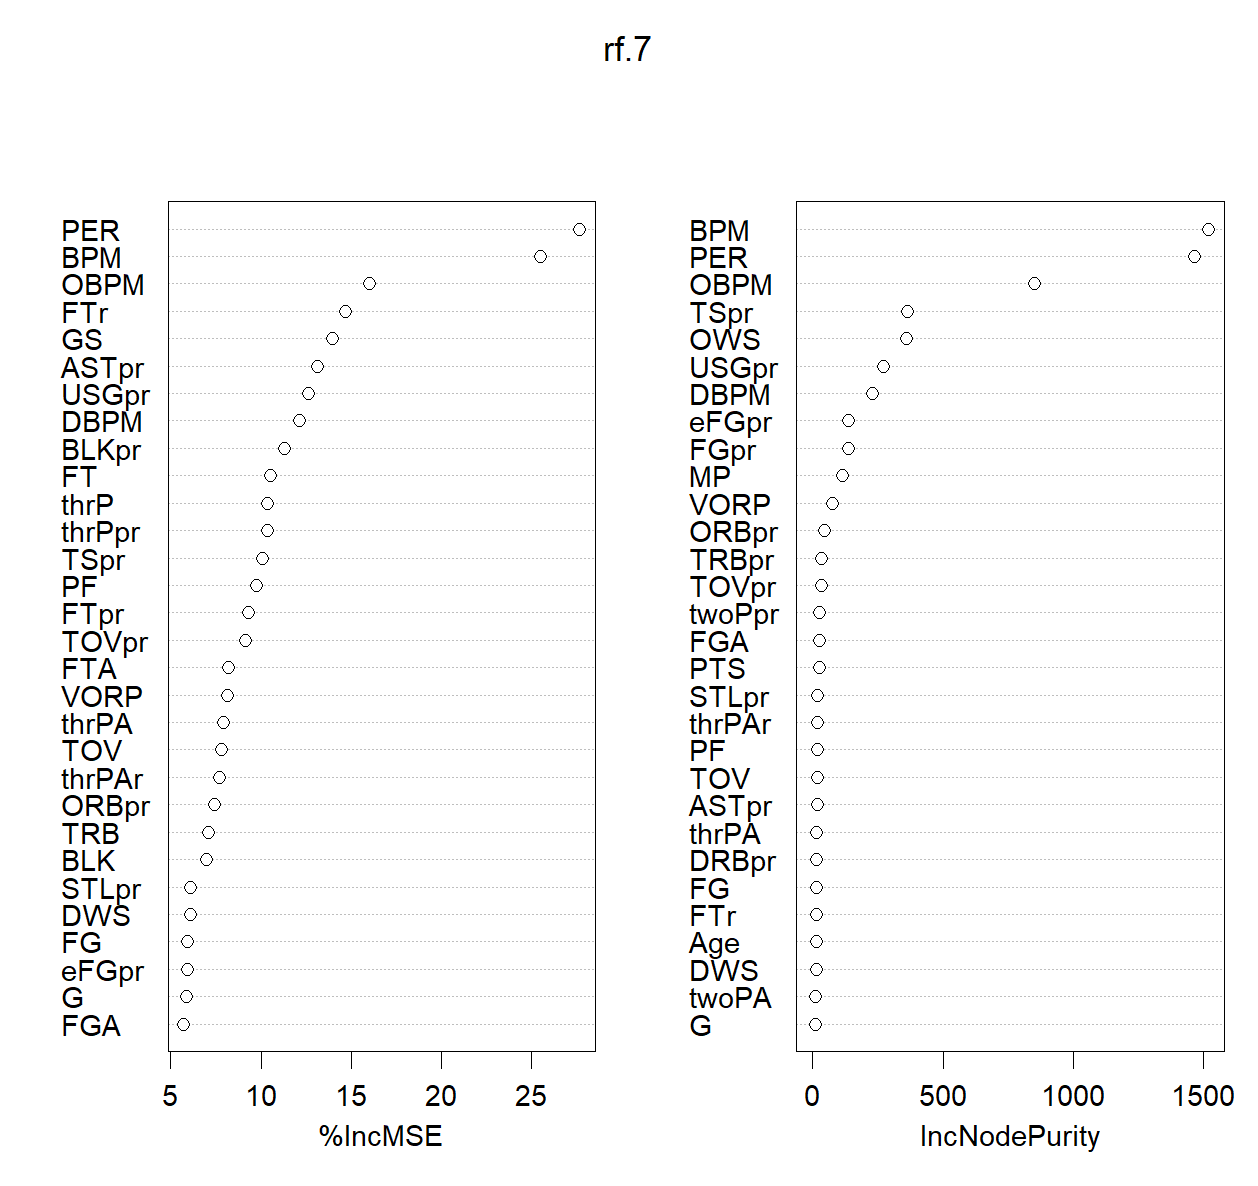
\includegraphics[width=0.4\textwidth]{rfera3}\hspace{1cm}
%\vspace{-1.9cm}
\caption{The three eras using Random Forest to determine the most important variables. \label{fig6}}
\end{figure} \leavevmode\\
As shown above, are the outputs of the three eras when run under Random Forest. From this, we can tell that the most critical variables are BPM and PER. BPM and PER were the important standard variables throughout the observations. Whether we looked at the worst or best teams, BPM and PER always came out on top. This caught our eye because, in the basketball community, PER, without context, is considered an alarming stat to base performance on. Since PER only looks at how an individual does and not necessarily their impact. It was interesting to see that a stat shouldn’t be valued independently as a predictor of how much they contribute to winning. But it was discovered that those variables are highly correlated. Thus, when running the Lasso, we had to run it for two separate events. Event one would be when BPM is the primary variable, thus eliminating all correlated variables toward BPM. Event two is when we concentrated on PER and eliminated the correlated variables with PER. As for PCR, we included all variables in the prediction model as correlations do not affect the method. \\\\
\indent When comparing the three methods, we used the RMSE, Root Mean Square Error, to determine the most accurate method for each observation. The results are as follows:\\
\begin{center}
\begin{tabular}{cc|c|c|c|c|l}
\cline{3-6}
& & \multicolumn{4}{ c| }{Methods: RMSE} \\ \cline{3-6}
& & Random Forest  & \multicolumn{2}{ c| }{Lasso} & PCR \\ \cline{4-5}&& & BPM & PER & \\ \cline{1-6} \cline{5-6}
\multicolumn{1}{ |c  }{\multirow{3}{*}{ERA 1} } &
\multicolumn{1}{ |c| }{Total} & 0.446 & 0.215 & 0.215 & 0.407 \\ \cline{2-6}
\multicolumn{1}{ |c  }{}                        &
\multicolumn{1}{ |c| }{Top 10} & 0.262 & 0.411 & 0.248 & 0.296 \\ \cline{2-6}
\multicolumn{1}{ |c  }{}                        &
\multicolumn{1}{ |c| }{Bottom 10} & 0.341 & 0.349 & 0.1922 & 0.2666 \\ \cline{1-6}
\multicolumn{1}{ |c  }{\multirow{3}{*}{ERA 2} } &
\multicolumn{1}{ |c| }{Total} & 0.334 & 0.2017 & 0.2204 & 0.201  \\ \cline{2-6}
\multicolumn{1}{ |c  }{}                        &
\multicolumn{1}{ |c| }{Top 10} & 0.346 & 0.182 & 0.188 & 0.157 \\ \cline{2-6}
\multicolumn{1}{ |c  }{}                        &
\multicolumn{1}{ |c| }{Bottom 10} & 0.397 & 0.367 & 0.219 & 0.293  \\ \cline{1-6}
\multicolumn{1}{ |c  }{\multirow{3}{*}{ERA 3} } &
\multicolumn{1}{ |c| }{Total} & 0.255 & 0.375 & 0.212 & 0.209 \\ \cline{2-6}
\multicolumn{1}{ |c  }{}                        &
\multicolumn{1}{ |c| }{Top 10} & 0.611 & 0.536 & 0.258 & 0.424 \\ \cline{2-6}
\multicolumn{1}{ |c  }{}                        &
\multicolumn{1}{ |c| }{Bottom 10} & 0.34 & 0.237 & 0.164 & 0.227 \\ \cline{1-6}
\end{tabular}
\end{center} \leavevmode \\

As we can see from the chart, Lasso was the best predictor for Era 1, whereas PCR was the best method for Era 2 and 3. Interestingly, Random Forest has a large RMSE compared to the other methods. This shows that in our dataset, random forest does not seem to be a suitable prediction method. This may have been because we standardized the data set. This may have skewed random forest results, but we decided to have the dataset standardized for all methods involved for consistency. It is also interesting how lasso, using PER, has some of the lowest RMSE of the results. As stated above, PER is not widely used to determine a player’s quality, but it seems better than BPM in deciding how much a player helps to win. Thus, it appears in the current landscape that it would be best to use PCR or lasso to predict if a player's stats represent how much they contribute to winning.

\newpage \noindent \textbf{Conclusion}\\\\

%Explain each method\\

Chapter 1:\\\\
\indent The conclusion for whether height determines how well a player is and as well if it will diminish over time is that it will not. We could only examine the relationship between height and weight in linear regression. Although this does not impact a player's performance, we can still see that the taller a player gets, the heavier they become.\\
\indent Next, we saw the use of quantile regression in our data. We looked at two different aspects, one was just for USA-born players, and the second was when the data were averaged per player basis. In this section, we looked at True shooting percentage and usage percentage. This should indicate if height gave a player a better advantage in shooting and how much they were used. We saw that the taller players were not used as much for the US players but were shooting the ball better than shorter players. This will be the same result when we average the player's stats. Thus we can say that taller players were not utilized enough for how well they were shooting.\\
\indent In Poisson regression, we used all the teams for all seasons and one team for all the seasons. This is where we started to see the lack of evidence for height affecting performance. For points, only 5 out of 30 teams had significance in height, and all five resulted in a negative coefficient. As for rebounds, about half the teams had significance, and they were positively coefficient. The only surprising factor here would be that only half teams had significance in rebounds. This would mean that taller players on these teams needed to be rebounding better, or the smaller players were good rebounders in their own right. However, when looking at one team through all seasons, is when a pattern emerges. In the case of The Los Angeles Lakers, only 9 of the 25 seasons resulted in significance. Moreover, most of those nine were due to the Lakers having one of the most dominating forces in the league. Therefore, throughout the lakers career, they have evenly spread in scoring. In scoring, we saw that it only mattered when the team had a presence to demand many points. The pattern of no significance is one we will look into further with GAM.\\
\indent After using GAM on the dataset, it was concluded that a player’ how well a player performs. This also answers whether the big players will disappear over time. Since it was concluded that height merely determines a particular player’s advantage, it does not make a player better. The determination for how good a player performs is how much effort they put into their work. An NBA player can be the shortest on the court by a wide margin and still act as if there is no height difference. For example, the player named Isaiah Thomas was almost an entire foot below league average in height. Yet that did not stop him from being one of the best players in the league for some seasons. This also goes for big players; no matter how big or tall they are, they can always be terrible if they do not have the skill set to become an NBA player.\\ \\

Chapter 2:\\\\

The conclusion for this chapter is that what determines how you win is BPM and PER. This is exciting because none of the small stats were as crucial as scoring or defense metrics. Usually, which player scored the most would have the most impact on winning. But that is not the case. It is not just about scoring. It is how that player is scoring. How efficient they are scoring and whether the points they score even matter. That’s where BPM and PER come in; BPM showcases the player’s impact while playing on the court. BPM considers scoring and how well the team plays while they play. If a player is only good on offense but terrible on defense, they might have low BPM, Because they are not contributing on the defensive end. PER will show how efficient the player is. If a player has to shoot a plethora of shoots to score an average amount, they might have a low PER since they are wasting possessions by shooting when they do not have to. Although we are a bit surprised that no other variables came close to being as crucial as BPM and PER, it does make sense why those two would be the best options to determine how helpful a player is at winning.

\newpage
\noindent \textbf{Future}\\\\
\indent What could be done in the future is a wide range of ideas. There are many different analytic resources and different variables to analyze. One variable we would like to focus on is called Raptor, created by the 538 analytical group. Raptor is like BPM, except it includes the player’s play-by-play in its data form. This means that Raptor would be an even more accurate form of determining the performance of a single player. In the future, we would like to merge Raptor with the data we have already and notice if there are any different interactions. Also, we would like to use other metrics when performing this same analysis. In this report, for chapter 2, we used a player’s culmination of a season. But there are many variations of how data is represented, such as per 100 possessions, per game, and per 36 minutes, to name a few. We would like to see how this different variant would impact how much a player contributes to winning.\\\\
\indent Another aspect to investigate is how individual teams determine what players to attract to win or lose. Whether there is a team that has been failing for many years or changes from losing to winning in an instant or vice versa, it would be what type of players teams look for when they want to win and succeed or when they try to win and fail. Usually, if a team wants to win, they will not necessarily go for players that score the most, rather than players that can play a particular style they want. It would also be interesting to see how salary affects these decisions. From how much a team can pay a player and if what they got paid was worth their output on the court.

\newpage
\bibliographystyle{plain}
\bibliography{ref}

\newpage \noindent \textbf{APPENDIX}\\\\
\textbf{DATA}\\
\noindent Chapter 1:\\
\textbf{Players name}: the name of players\\
\textbf{Team Abbreviation}: The abbreviation of the teams that the player played for\\
\textbf{College}: The college that player attended\\
\textbf{Country}: The country the player is from\\
\textbf{Draft year}: The year that player was drafted\\
\textbf{Draft round}: The round that player was drafter in\\
\textbf{Draft number}: The number the player was drafted in their respective round\\
\textbf{Season}: The season in which that player and the respective variable values happened\\

\noindent The numerical variables are as follows:\\
\textbf{X}: The index of each player\\
\textbf{Age}: The age the player during that season\\
\textbf{Player weight}: The weight of that player for that season\\
\textbf{Games Played}: The number of games played for that player during that season\\
\textbf{Net Rating}: The teams point differential per 100 possessions for that player during that season\\
\textbf{Offensive rebound percentage}: The percent for offensive rebound for that player during that season\\
\textbf{Defensive rebound percentage}: The percent for defensive rebound for that player during that season\\
\textbf{Assists}: The average number of assists per game for that player during that season\\
\textbf{Assist percentage}: The percent of field goals that player assisted on during that season\\
\textbf{Offensive rebound percentage}: The percent for offensive rebound for that player during that season\\
\cite{1} \leavevmode \newline\\\\
Chapter 2:\\\\
\textbf{Player:} The players name\\
\textbf{Pos:} The position of the player\\
\textbf{Age:} The age of the player in that season\\
\textbf{Tm:} The team the players played for in that season\\
\textbf{G:} Games played that season\\
\textbf{GS:} Games started that season\\
\textbf{MP:} Minutes played that season\\
\textbf{FG:} Field goals made that season\\
\textbf{FGA:} Field goal attempts during that season\\
\textbf{FG Percent:} Field goal percentage during that season\\
\textbf{3P:} Three pointers made that season\\
\textbf{3PA:} Three point attempts during that season\\
\textbf{3PA Percent:} Three point percentage during that season\\
\textbf{2P:} Two pointers made during that season\\
\textbf{2PA:} Two point attempts during that season\\
\textbf{2P Percent:} Two point percentage during that season\\
\textbf{eFG Percent:} Field goal percentage that adjusts the fact that three point field goal is worth more than two\\
\textbf{FT:} Free throws made in a season\\
\textbf{FTA:} Free throw attempts in the season\\
\textbf{FT Percent:} Free throw percentage during the season\\
\textbf{ORB:} Offensive rebounds during that season\\
\textbf{DRB:} Defensive rebounds during that season\\
\textbf{TRB:} Total rebounds during that season\\
\textbf{AST:} Total assists during that season\\
\textbf{STL:} Total steals during that season\\
\textbf{BLK:} Total blocks during that season\\
\textbf{TOV:} Total turnovers during that season\\
\textbf{PF:} Total personal fouls during that season\\
\textbf{PTS:} Total points during that season\\
\textbf{TS Percentage:} Measure of Shooting efficiency that takes into account two point field goals, three point field goals, and free throws\\
\textbf{3PAr:} Percentage of FG attempts from three point range\\
\textbf{FTr:} Number of FT attempts per FG attempt\\
\textbf{ORB Percent:} Percentage of available offensive rebounds a player grabbed while they were on the floor\\
\textbf{DRB Percent:} Percentage of available defensive rebounds a player grabbed while they were on the floor\\
\textbf{TRB Percent:} An estimate of the percentage of available rebounds a player grabbed while they were on the floor\\
\textbf{AST Percent:} Percentage of teammate field goals a player assisted while they were on the floor\\
\textbf{STL Percent:} Percentage of opponent possessions that end with a steal by the player while they were on the floor\\
\textbf{BLK Percent:} An estimate of the percentage of opponent two point field goal attempts blocked while on the floor\\
\textbf{TOV Percent:} Turnovers committed per 100 plays\\
\textbf{USG Percent:} Percentage of team plays used by a player while they were on the floor\\
\textbf{OWS:} Number of wins contributed by a player due to offense\\
\textbf{DWS:} Number of wins contributed by a player due to defense\\
\textbf{WS:} Number of wins contributed by a player\\
\textbf{OBPM:} Box score estimate of the offensive points per 100 possessions a player contributed above a league average player\\
\textbf{DPM:} Box score estimate of the defensive points per 100 possessions a player contributed above a league average player\\
\textbf{VORP:} Box score estimate of points per 100 TEAM possessions that a player contributed above a replacements level player\\
\cite{6} \leavevmode \newline\\\\
\newpage
\textbf{CODE:}\\
%\begin{verbatim}
\begin{lstlisting}[breaklines]
nba = read.csv("~/math/data/all_seasons.csv")

lm.fit2=lm(nbau$player_weight~nbau$player_height)

summary(lm.fit2)
plot(lm.fit2)
lm.fit2=lm(nbau$ts_pct~nbau$player_height)
summary(lm.fit2)
plot(lm.fit2)
summary(rqfit90 <- rq(nbau$ts_pct~nbau$player_height, tau = 0.90))
summary(rqfit90 <- rq(nbau$usg_pct~nbau$player_height, tau = 0.90))
summary(rqfit90 <- rq(nba.players$ts_pct~nba.players$player_height, tau = 0.95))
summary(rqfit90 <- rq(nba.players$usg_pct~nba.players$player_height, tau = 0.90))
#######################
##  ALL TEAM ONE SEASON##
#######################

nba.season10=nba[which(nba$season=="2009-10"),]
summary(nba.season10$team_abbreviation)

nba.season10ATL=nba[which(nba$season=="2009-10" & nba$team_abbreviation=="ATL"),]
plot(nba.season10ATL$player_height,nba.season10ATL$reb )
text(nba.season10ATL$player_height, nba.season10ATL$reb, nba.season10ATL$player_name)
x.atlreb<-summary(m1 <- glm(nba.season10ATL$reb ~ nba.season10ATL$player_height, family="poisson"))
x.atlpts<-summary(m1 <- glm(nba.season10ATL$pts ~ nba.season10ATL$player_height, family="poisson"))

nba.season10BOS=nba[which(nba$season=="2009-10" & nba$team_abbreviation=="BOS"),]
x.bosreb<-summary(m1 <- glm(nba.season10BOS$reb ~ nba.season10BOS$player_height, family="poisson"))
x.bospts<-summary(m1 <- glm(nba.season10BOS$pts ~ nba.season10BOS$player_height, family="poisson"))

nba.season10CHA=nba[which(nba$season=="2009-10" & nba$team_abbreviation=="CHA"),]
x.chareb<-summary(m1 <- glm(nba.season10CHA$reb ~ nba.season10CHA$player_height, family="poisson"))
x.chapts<-summary(m1 <- glm(nba.season10CHA$pts ~ nba.season10CHA$player_height, family="poisson"))

nba.season10CHI=nba[which(nba$season=="2009-10" & nba$team_abbreviation=="CHI"),]
x.chireb<-summary(m1 <- glm(nba.season10CHI$reb ~ nba.season10CHI$player_height, family="poisson"))
x.chipts<-summary(m1 <- glm(nba.season10CHI$pts ~ nba.season10CHI$player_height, family="poisson"))

nba.season10CLE=nba[which(nba$season=="2009-10" & nba$team_abbreviation=="CLE"),]
x.clereb<-summary(m1 <- glm(nba.season10CLE$reb ~ nba.season10CLE$player_height, family="poisson"))
x.clepts<-summary(m1 <- glm(nba.season10CLE$pts ~ nba.season10CLE$player_height, family="poisson"))

nba.season10DAL=nba[which(nba$season=="2009-10" & nba$team_abbreviation=="DAL"),]
x.dalreb<-summary(m1 <- glm(nba.season10DAL$reb ~ nba.season10DAL$player_height, family="poisson"))
x.dalpts<-summary(m1 <- glm(nba.season10DAL$pts ~ nba.season10DAL$player_height, family="poisson"))

nba.season10DEN=nba[which(nba$season=="2009-10" & nba$team_abbreviation=="DEN"),]
x.denreb<-summary(m1 <- glm(nba.season10DEN$reb ~ nba.season10DEN$player_height, family="poisson"))
x.denpts<-summary(m1 <- glm(nba.season10DEN$pts ~ nba.season10DEN$player_height, family="poisson"))

nba.season10DET=nba[which(nba$season=="2009-10" & nba$team_abbreviation=="DET"),]
x.detreb<-summary(m1 <- glm(nba.season10DET$reb ~ nba.season10DET$player_height, family="poisson"))
x.detpts<-summary(m1 <- glm(nba.season10DET$pts ~ nba.season10DET$player_height, family="poisson"))

nba.season10GSW=nba[which(nba$season=="2009-10" & nba$team_abbreviation=="GSW"),]
x.gswreb<-summary(m1 <- glm(nba.season10GSW$reb ~ nba.season10GSW$player_height, family="poisson"))
x.gswpts<-summary(m1 <- glm(nba.season10GSW$pts ~ nba.season10GSW$player_height, family="poisson"))

nba.season10HOU=nba[which(nba$season=="2009-10" & nba$team_abbreviation=="HOU"),]
x.houreb<-summary(m1 <- glm(nba.season10HOU$reb ~ nba.season10HOU$player_height, family="poisson"))
x.houpts<-summary(m1 <- glm(nba.season10HOU$pts ~ nba.season10HOU$player_height, family="poisson"))

nba.season10IND=nba[which(nba$season=="2009-10" & nba$team_abbreviation=="IND"),]
x.indreb<-summary(m1 <- glm(nba.season10IND$reb ~ nba.season10IND$player_height, family="poisson"))
x.indpts<-summary(m1 <- glm(nba.season10IND$pts ~ nba.season10IND$player_height, family="poisson"))

nba.season10LAC=nba[which(nba$season=="2009-10" & nba$team_abbreviation=="LAC"),]
x.lacreb<-summary(m1 <- glm(nba.season10LAC$reb ~ nba.season10LAC$player_height, family="poisson"))
x.lacpts<-summary(m1 <- glm(nba.season10LAC$pts ~ nba.season10LAC$player_height, family="poisson"))

nba.season10LAL=nba[which(nba$season=="2009-10" & nba$team_abbreviation=="LAL"),]
x.lalreb<-summary(m1 <- glm(nba.season10LAL$reb ~ nba.season10LAL$player_height, family="poisson"))
x.lalpts<-summary(m1 <- glm(nba.season10LAL$pts ~ nba.season10LAL$player_height, family="poisson"))

nba.season10MEM=nba[which(nba$season=="2009-10" & nba$team_abbreviation=="MEM"),]
x.memreb<-summary(m1 <- glm(nba.season10MEM$reb ~ nba.season10MEM$player_height, family="poisson"))
x.mempts<-summary(m1 <- glm(nba.season10MEM$pts ~ nba.season10MEM$player_height, family="poisson"))

nba.season10MIA=nba[which(nba$season=="2009-10" & nba$team_abbreviation=="MIA"),]
x.miareb<-summary(m1 <- glm(nba.season10MIA$reb ~ nba.season10MIA$player_height, family="poisson"))
x.miapts<-summary(m1 <- glm(nba.season10MIA$pts ~ nba.season10MIA$player_height, family="poisson"))

nba.season10MIL=nba[which(nba$season=="2009-10" & nba$team_abbreviation=="MIL"),]
x.milreb<-summary(m1 <- glm(nba.season10MIL$reb ~ nba.season10MIL$player_height, family="poisson"))
x.milpts<-summary(m1 <- glm(nba.season10MIL$pts ~ nba.season10MIL$player_height, family="poisson"))

nba.season10MIN=nba[which(nba$season=="2009-10" & nba$team_abbreviation=="MIN"),]
x.minreb<-summary(m1 <- glm(nba.season10MIN$reb ~ nba.season10MIN$player_height, family="poisson"))
x.minpts<-summary(m1 <- glm(nba.season10MIN$pts ~ nba.season10MIN$player_height, family="poisson"))

nba.season10NJN=nba[which(nba$season=="2009-10" & nba$team_abbreviation=="NJN"),]
x.njnreb<-summary(m1 <- glm(nba.season10NJN$reb ~ nba.season10NJN$player_height, family="poisson"))
x.njnpts<-summary(m1 <- glm(nba.season10NJN$pts ~ nba.season10NJN$player_height, family="poisson"))

nba.season10NOH=nba[which(nba$season=="2009-10" & nba$team_abbreviation=="NOH"),]
x.nohreb<-summary(m1 <- glm(nba.season10NOH$reb ~ nba.season10NOH$player_height, family="poisson"))
x.nohpts<-summary(m1 <- glm(nba.season10NOH$pts ~ nba.season10NOH$player_height, family="poisson"))

nba.season10NYK=nba[which(nba$season=="2009-10" & nba$team_abbreviation=="NYK"),]
x.nykreb<-summary(m1 <- glm(nba.season10NYK$reb ~ nba.season10NYK$player_height, family="poisson"))
x.nykpts<-summary(m1 <- glm(nba.season10NYK$pts ~ nba.season10NYK$player_height, family="poisson"))

nba.season10OKC=nba[which(nba$season=="2009-10" & nba$team_abbreviation=="OKC"),]
x.okcreb<-summary(m1 <- glm(nba.season10OKC$reb ~ nba.season10OKC$player_height, family="poisson"))
x.okcpts<-summary(m1 <- glm(nba.season10OKC$pts ~ nba.season10OKC$player_height, family="poisson"))

nba.season10ORL=nba[which(nba$season=="2009-10" & nba$team_abbreviation=="ORL"),]
x.orlreb<-summary(m1 <- glm(nba.season10ORL$reb ~ nba.season10ORL$player_height, family="poisson"))
x.orlpts<-summary(m1 <- glm(nba.season10ORL$pts ~ nba.season10ORL$player_height, family="poisson"))

nba.season10PHI=nba[which(nba$season=="2009-10" & nba$team_abbreviation=="PHI"),]
x.phireb<-summary(m1 <- glm(nba.season10PHI$reb ~ nba.season10PHI$player_height, family="poisson"))
x.phipts<-summary(m1 <- glm(nba.season10PHI$pts ~ nba.season10PHI$player_height, family="poisson"))

nba.season10PHX=nba[which(nba$season=="2009-10" & nba$team_abbreviation=="PHX"),]
x.phxreb<-summary(m1 <- glm(nba.season10PHX$reb ~ nba.season10PHX$player_height, family="poisson"))
x.phxpts<-summary(m1 <- glm(nba.season10PHX$pts ~ nba.season10PHX$player_height, family="poisson"))

nba.season10POR=nba[which(nba$season=="2009-10" & nba$team_abbreviation=="POR"),]
x.porreb<-summary(m1 <- glm(nba.season10POR$reb ~ nba.season10POR$player_height, family="poisson"))
x.porpts<-summary(m1 <- glm(nba.season10POR$pts ~ nba.season10POR$player_height, family="poisson"))

nba.season10SAC=nba[which(nba$season=="2009-10" & nba$team_abbreviation=="SAC"),]
x.sacreb<-summary(m1 <- glm(nba.season10SAC$reb ~ nba.season10SAC$player_height, family="poisson"))
x.sacpts<-summary(m1 <- glm(nba.season10SAC$pts ~ nba.season10SAC$player_height, family="poisson"))

nba.season10SAS=nba[which(nba$season=="2009-10" & nba$team_abbreviation=="SAS"),]
x.sasreb<-summary(m1 <- glm(nba.season10SAS$reb ~ nba.season10SAS$player_height, family="poisson"))
x.saspts<-summary(m1 <- glm(nba.season10SAS$pts ~ nba.season10SAS$player_height, family="poisson"))

nba.season10TOR=nba[which(nba$season=="2009-10" & nba$team_abbreviation=="TOR"),]
x.torreb<-summary(m1 <- glm(nba.season10TOR$reb ~ nba.season10TOR$player_height, family="poisson"))
x.torpts<-summary(m1 <- glm(nba.season10TOR$pts ~ nba.season10TOR$player_height, family="poisson"))

nba.season10UTA=nba[which(nba$season=="2009-10" & nba$team_abbreviation=="UTA"),]
x.utareb<-summary(m1 <- glm(nba.season10UTA$reb ~ nba.season10UTA$player_height, family="poisson"))
x.utapts<-summary(m1 <- glm(nba.season10UTA$pts ~ nba.season10UTA$player_height, family="poisson"))

nba.season10WAS=nba[which(nba$season=="2009-10" & nba$team_abbreviation=="WAS"),]
x.wasreb<-summary(m1 <- glm(nba.season10WAS$reb ~ nba.season10WAS$player_height, family="poisson"))
x.waspts<-summary(m1 <- glm(nba.season10WAS$pts ~ nba.season10WAS$player_height, family="poisson"))

data.frame(x.clereb$coefficients,x.dalreb$coefficients,x.denreb$coefficients,x.detreb$coefficients,x.gswreb$coefficients,
                 x.houreb$coefficients)
x.atlreb$coefficients
x.bosreb$coefficients
x.chareb$coefficients
x.chireb$coefficients
x.clereb$coefficients
x.dalreb$coefficients
x.denreb$coefficients
x.detreb$coefficients
x.gswreb$coefficients
x.houreb$coefficients
x.indreb$coefficients
x.lacreb$coefficients
x.lalreb$coefficients
x.memreb$coefficients
x.miareb$coefficients
x.milreb$coefficients
x.minreb$coefficients
x.njnreb$coefficients
x.nohreb$coefficients
x.nykreb$coefficients
x.okcreb$coefficients
x.orlreb$coefficients
x.phireb$coefficients
x.phxreb$coefficients
x.porreb$coefficients
x.sacreb$coefficients
x.sasreb$coefficients
x.torreb$coefficients
x.utareb$coefficients
x.wasreb$coefficients

x.atlpts$coefficients
x.bospts$coefficients
x.chapts$coefficients
x.chipts$coefficients
x.clepts$coefficients
x.dalpts$coefficients
x.denpts$coefficients
x.detpts$coefficients
x.gswpts$coefficients
x.houpts$coefficients
x.indpts$coefficients
x.lacpts$coefficients
x.lalpts$coefficients
x.mempts$coefficients
x.miapts$coefficients
x.milpts$coefficients
x.minpts$coefficients
x.njnpts$coefficients
x.nohpts$coefficients
x.nykpts$coefficients
x.okcpts$coefficients
x.orlpts$coefficients
x.phipts$coefficients
x.phxpts$coefficients
x.porpts$coefficients
x.sacpts$coefficients
x.saspts$coefficients
x.torpts$coefficients
x.utapts$coefficients
x.waspts$coefficients

#######################
##  ONE TEAM ALL SEASONS##
#######################


#BEST points & BEST rebounds
nba.LAL=nba[which(nba$team_abbreviation=="LAL"),]

plot(nba.LAL$player_height,nba.LAL$reb )
text(nba.LAL$player_height, nba.LAL$reb, nba.LAL$player_name)


as.integer(nba.LAL97$reb) 
nba.LAL97=nba.LAL[which(nba.LAL$season=="1996-97"),]
(x.LAL97reb<-summary(m1 <- glm(nba.LAL97$reb ~ nba.LAL97$player_height, family="poisson")))
x.LAL97pts<-summary(m1 <- glm(nba.LAL97$pts ~ nba.LAL97$player_height, family="poisson"))
x.LAL97reb$coefficients

nba.LAL98=nba.LAL[which(nba.LAL$season=="1997-98"),]
x.LAL98reb<-summary(m1 <- glm(nba.LAL98$reb ~ nba.LAL98$player_height, family="poisson"))
x.LAL98pts<-summary(m1 <- glm(nba.LAL98$pts ~ nba.LAL98$player_height, family="poisson"))

nba.LAL99=nba.LAL[which(nba.LAL$season=="1998-99"),]
x.LAL99reb<-summary(m1 <- glm(nba.LAL99$reb ~ nba.LAL99$player_height, family="poisson"))
x.LAL99pts<-summary(m1 <- glm(nba.LAL99$pts ~ nba.LAL99$player_height, family="poisson"))

nba.LAL00=nba.LAL[which(nba.LAL$season=="1999-00"),]
x.LAL00reb<-summary(m1 <- glm(nba.LAL00$reb ~ nba.LAL00$player_height, family="poisson"))
x.LAL00pts<-summary(m1 <- glm(nba.LAL00$pts ~ nba.LAL00$player_height, family="poisson"))

nba.LAL01=nba.LAL[which(nba.LAL$season=="2000-01"),]
x.LAL01reb<-summary(m1 <- glm(nba.LAL01$reb ~ nba.LAL01$player_height, family="poisson"))
x.LAL01pts<-summary(m1 <- glm(nba.LAL01$pts ~ nba.LAL01$player_height, family="poisson"))

nba.LAL02=nba.LAL[which(nba.LAL$season=="2001-02"),]
x.LAL02reb<-summary(m1 <- glm(nba.LAL02$reb ~ nba.LAL02$player_height, family="poisson"))
x.LAL02pts<-summary(m1 <- glm(nba.LAL02$pts ~ nba.LAL02$player_height, family="poisson"))

nba.LAL03=nba.LAL[which(nba.LAL$season=="2002-03"),]
x.LAL03reb<-summary(m1 <- glm(nba.LAL03$reb ~ nba.LAL03$player_height, family="poisson"))
x.LAL03pts<-summary(m1 <- glm(nba.LAL03$pts ~ nba.LAL03$player_height, family="poisson"))

nba.LAL04=nba.LAL[which(nba.LAL$season=="2003-04"),]
x.LAL04reb<-summary(m1 <- glm(nba.LAL04$reb ~ nba.LAL04$player_height, family="poisson"))
x.LAL04pts<-summary(m1 <- glm(nba.LAL04$pts ~ nba.LAL04$player_height, family="poisson"))

nba.LAL05=nba.LAL[which(nba.LAL$season=="2004-05"),]
x.LAL05reb<-summary(m1 <- glm(nba.LAL05$reb ~ nba.LAL05$player_height, family="poisson"))
x.LAL05pts<-summary(m1 <- glm(nba.LAL05$pts ~ nba.LAL05$player_height, family="poisson"))

nba.LAL06=nba.LAL[which(nba.LAL$season=="2005-06"),]
x.LAL06reb<-summary(m1 <- glm(nba.LAL06$reb ~ nba.LAL06$player_height, family="poisson"))
x.LAL06pts<-summary(m1 <- glm(nba.LAL06$pts ~ nba.LAL06$player_height, family="poisson"))

nba.LAL07=nba.LAL[which(nba.LAL$season=="2006-07"),]
x.LAL07reb<-summary(m1 <- glm(nba.LAL07$reb ~ nba.LAL07$player_height, family="poisson"))
x.LAL07pts<-summary(m1 <- glm(nba.LAL07$pts ~ nba.LAL07$player_height, family="poisson"))

nba.LAL08=nba.LAL[which(nba.LAL$season=="2007-08"),]
x.LAL08reb<-summary(m1 <- glm(nba.LAL08$reb ~ nba.LAL08$player_height, family="poisson"))
x.LAL08pts<-summary(m1 <- glm(nba.LAL08$pts ~ nba.LAL08$player_height, family="poisson"))

nba.LAL09=nba.LAL[which(nba.LAL$season=="2008-09"),]
x.LAL09reb<-summary(m1 <- glm(nba.LAL09$reb ~ nba.LAL09$player_height, family="poisson"))
x.LAL09pts<-summary(m1 <- glm(nba.LAL09$pts ~ nba.LAL09$player_height, family="poisson"))

nba.LAL10=nba.LAL[which(nba.LAL$season=="2009-10"),]
x.LAL10reb<-summary(m1 <- glm(nba.LAL10$reb ~ nba.LAL10$player_height, family="poisson"))
x.LAL10pts<-summary(m1 <- glm(nba.LAL10$pts ~ nba.LAL10$player_height, family="poisson"))

nba.LAL11=nba.LAL[which(nba.LAL$season=="2010-11"),]
x.LAL11reb<-summary(m1 <- glm(nba.LAL11$reb ~ nba.LAL11$player_height, family="poisson"))
x.LAL11pts<-summary(m1 <- glm(nba.LAL11$pts ~ nba.LAL11$player_height, family="poisson"))

nba.LAL12=nba.LAL[which(nba.LAL$season=="2011-12"),]
x.LAL12reb<-summary(m1 <- glm(nba.LAL12$reb ~ nba.LAL12$player_height, family="poisson"))
x.LAL12pts<-summary(m1 <- glm(nba.LAL12$pts ~ nba.LAL12$player_height, family="poisson"))

nba.LAL13=nba.LAL[which(nba.LAL$season=="2012-13"),]
x.LAL13reb<-summary(m1 <- glm(nba.LAL13$reb ~ nba.LAL13$player_height, family="poisson"))
x.LAL13pts<-summary(m1 <- glm(nba.LAL13$pts ~ nba.LAL13$player_height, family="poisson"))

nba.LAL14=nba.LAL[which(nba.LAL$season=="2013-14"),]
x.LAL14reb<-summary(m1 <- glm(nba.LAL14$reb ~ nba.LAL14$player_height, family="poisson"))
x.LAL14pts<-summary(m1 <- glm(nba.LAL14$pts ~ nba.LAL14$player_height, family="poisson"))

nba.LAL15=nba.LAL[which(nba.LAL$season=="2014-15"),]
x.LAL15reb<-summary(m1 <- glm(nba.LAL15$reb ~ nba.LAL15$player_height, family="poisson"))
x.LAL15pts<-summary(m1 <- glm(nba.LAL15$pts ~ nba.LAL15$player_height, family="poisson"))

nba.LAL16=nba.LAL[which(nba.LAL$season=="2015-16"),]
x.LAL16reb<-summary(m1 <- glm(nba.LAL16$reb ~ nba.LAL16$player_height, family="poisson"))
x.LAL16pts<-summary(m1 <- glm(nba.LAL16$pts ~ nba.LAL16$player_height, family="poisson"))

nba.LAL17=nba.LAL[which(nba.LAL$season=="2016-17"),]
x.LAL17reb<-summary(m1 <- glm(nba.LAL17$reb ~ nba.LAL17$player_height, family="poisson"))
x.LAL17pts<-summary(m1 <- glm(nba.LAL17$pts ~ nba.LAL17$player_height, family="poisson"))

nba.LAL18=nba.LAL[which(nba.LAL$season=="2017-18"),]
x.LAL18reb<-summary(m1 <- glm(nba.LAL18$reb ~ nba.LAL18$player_height, family="poisson"))
x.LAL18pts<-summary(m1 <- glm(nba.LAL18$pts ~ nba.LAL18$player_height, family="poisson"))

nba.LAL19=nba.LAL[which(nba.LAL$season=="2018-19"),]
x.LAL19reb<-summary(m1 <- glm(nba.LAL19$reb ~ nba.LAL19$player_height, family="poisson"))
x.LAL19pts<-summary(m1 <- glm(nba.LAL19$pts ~ nba.LAL19$player_height, family="poisson"))

nba.LAL20=nba.LAL[which(nba.LAL$season=="2019-20"),]
x.LAL20reb<-summary(m1 <- glm(nba.LAL20$reb ~ nba.LAL20$player_height, family="poisson"))
x.LAL20pts<-summary(m1 <- glm(nba.LAL20$pts ~ nba.LAL20$player_height, family="poisson"))

nba.LAL21=nba.LAL[which(nba.LAL$season=="2020-21"),]
x.LAL21reb<-summary(m1 <- glm(nba.LAL21$reb ~ nba.LAL21$player_height, family="poisson"))
x.LAL21pts<-summary(m1 <- glm(nba.LAL21$pts ~ nba.LAL21$player_height, family="poisson"))


x.LAL97reb$coefficients
x.LAL98reb$coefficients
x.LAL99reb$coefficients
x.LAL00reb$coefficients
x.LAL01reb$coefficients
x.LAL02reb$coefficients
x.LAL03reb$coefficients
x.LAL04reb$coefficients
x.LAL05reb$coefficients
x.LAL06reb$coefficients
x.LAL07reb$coefficients
x.LAL08reb$coefficients
x.LAL09reb$coefficients
x.LAL10reb$coefficients
x.LAL11reb$coefficients
x.LAL12reb$coefficients
x.LAL13reb$coefficients
x.LAL14reb$coefficients
x.LAL15reb$coefficients
x.LAL16reb$coefficients
x.LAL17reb$coefficients
x.LAL18reb$coefficients
x.LAL19reb$coefficients
x.LAL20reb$coefficients
x.LAL21reb$coefficients


x.LAL97pts$coefficients
x.LAL98pts$coefficients
x.LAL99pts$coefficients
x.LAL00pts$coefficients
x.LAL01pts$coefficients
x.LAL02pts$coefficients
x.LAL03pts$coefficients
x.LAL04pts$coefficients
x.LAL05pts$coefficients
x.LAL06pts$coefficients
x.LAL07pts$coefficients
x.LAL08pts$coefficients
x.LAL09pts$coefficients
x.LAL10pts$coefficients
x.LAL11pts$coefficients
x.LAL12pts$coefficients
x.LAL13pts$coefficients
x.LAL14pts$coefficients
x.LAL15pts$coefficients
x.LAL16pts$coefficients
x.LAL17pts$coefficients
x.LAL18pts$coefficients
x.LAL19pts$coefficients
x.LAL20pts$coefficients
x.LAL21pts$coefficients

plot(gam(nba.era1$pts ~ s(nba.era1$player_height), method="REML"))

plot(gam(nba.era2$pts ~ s(nba.era2$player_height), method="REML"))

plot(gam(nba.era3$pts ~ s(nba.era3$player_height), method="REML"))

plot(gam(nba.era1$ts_pct ~ s(nba.era1$player_height), method="REML"))

plot(gam(nba.era2$ts_pct ~ s(nba.era2$player_height), method="REML"))

plot(gam(nba.era3$ts_pct ~ s(nba.era3$player_height), method="REML"))

plot(gam(nba.era1$usg_pct ~ s(nba.era1$player_height), method="REML"))

plot(gam(nba.era2$usg_pct ~ s(nba.era2$player_height), method="REML"))

plot(gam(nba.era3$usg_pct ~ s(nba.era3$player_height), method="REML"))

Chapter 2:\\
##############################################
#ERA 1
############################################################################

####################################################
#Random forest (with outliers and standardization)

nbaera1.r = subset(nbaera1, select = -c(Rk,Player,Pos,Tm) )
nbaera1_r <- as.data.frame(scale(nbaera1.r[1:46]))

colnames(nbaera1_r) <- gsub("%", "pr", colnames(nbaera1_r))
colnames(nbaera1_r) <- gsub("2", "two", colnames(nbaera1_r))
colnames(nbaera1_r) <- gsub("3", "thr", colnames(nbaera1_r))
colnames(nbaera1_r) <- gsub("/48", "pfe", colnames(nbaera1_r))
nbaera1_r = subset(nbaera1_r, select = -c(WS) )

library(randomForest)

rf.1=randomForest(nbaera1_r$WSpfe ~ . ,data = nbaera1_r, importance=TRUE)
importance(rf.1)
varImpPlot(rf.1)

actual <- nbaera1_r$WSpfe
predicted <- unname(predict(rf.1, nbaera1_r))

R2 <- 1 - (sum((actual-predicted)^2)/sum((actual-mean(actual))^2))
R2

#R2= 0.9789


#Most important are 
#BIG: BPM, PER 
#Alittle less: DWS

cor(nbaera1_r$BPM,nbaera1_r$PER)

######################################
#Random forest prediction

y <- nbaera1_r$WSpfe
nbaera1_rf = subset(nbaera1_r, select = -c(WSpfe) )
x = data.matrix(nbaera1_rf)

set.seed(1)
train=sample(1:nrow(x), nrow(x)*.7)
test=(-train)
y.test=y[test]

set.seed(1)

rf=randomForest(WSpfe~.,data=nbaera1_r,subset=train,importance=TRUE)
varImpPlot(rf)
yhat = predict(rf,newdata=nbaera1_r[-train,])
plot(yhat, y.test)
abline(0,1)
sqrt(mean((yhat-y.test)^2))

#Random forest prediction: 0.446
#    Min.  1st Qu.   Median     Mean  3rd Qu.     Max. 
#-23.1987  -0.3041   0.1159   0.0000   0.4753  11.7148

#####################################

#######################
#Lasso

y <- nbaera1_r$WSpfe
nbaera1_L = subset(nbaera1_r, select = -c(WSpfe) )
x = data.matrix(nbaera1_L)

options(max.print=1936)
cor(x)

#BPM: PER, OBPM 
nbaera1_L = subset(nbaera1_r, select = -c(WSpfe, PER, OBPM) )
x = data.matrix(nbaera1_L)
#PER: TSpr, OBPM, BPM
nbaera1_L = subset(nbaera1_r, select = -c(WSpfe, BPM, OBPM, TSpr) )
x = data.matrix(nbaera1_L)

library(glmnet)

#perform k-fold cross-validation to find optimal lambda value
cv_model <- cv.glmnet(x, y, alpha = 1)

#find optimal lambda value that minimizes test MSE
#Min Lambda
best_lambda <- cv_model$lambda.min
#Max lambda to be within 1 standard error of the minimum
best_lambda <- cv_model$lambda.1se
best_lambda

print(cv_model)

#produce plot of test MSE by lambda value
plot(cv_model) 

best_model <- glmnet(x, y, alpha = 1, lambda = best_lambda)
coef(best_model)
#use fitted best model to make predictions
y_predicted <- predict(best_model, s = best_lambda, newx = x)

#find SST and SSE
sst <- sum((y - mean(y))^2)
sse <- sum((y_predicted - y)^2)

#find R-Squared
rsq <- 1 - sse/sst
rsq

#BPM: R2 = 0.9058

#PER: R2 = 0.9633

###################
#Lasso prediction

#BPM: PER, OBPM
nbaera1_L = subset(nbaera1_r, select = -c(WSpfe, PER, OBPM) )
x = data.matrix(nbaera1_L)
#PER: TSpr, OBPM, BPM
nbaera1_L = subset(nbaera1_r, select = -c(WSpfe, BPM, OBPM, TSpr) )
x = data.matrix(nbaera1_L)

y <- nbaera1_r$WSpfe
nbaera1_pcr = subset(nbaera1_r, select = -c(WSpfe) )
x = data.matrix(nbaera1_pcr)

set.seed(1)
train=sample(1:nrow(x), nrow(x)*.7)
test=(-train)
y.test=y[test]

library(glmnet)
lasso.mod=glmnet(x[train,],y[train],alpha=1)
plot(lasso.mod)#coefficient plot

set.seed(1)
cv.out=cv.glmnet(x[train,],y[train],alpha=1)
plot(cv.out)#CV error plot
bestlam=cv.out$lambda.1se
bestlam
lasso.pred=predict(lasso.mod,s=bestlam,newx=x[test,])
sqrt(mean((lasso.pred-y.test)^2))
summary(y)

#Based on test
#Prediction for BPM: 0.215
#Prediction for PER: 0.215

#    Min.  1st Qu.   Median     Mean  3rd Qu.     Max. 
#-23.1987  -0.3041   0.1159   0.0000   0.4753  11.7148

##########################################################
#PCR
library(pls)
#make this example reproducible
set.seed(1)

#fit PCR model Random Forrest
model <- pcr(nbaera1_r$WSpfe~.,data=nbaera1_r, scale=TRUE, validation="CV")
summary(model)

#Lasso BPM
model <- pcr(nbaera1_r$WSpfe~BPM+FTpr+TSpr+thrPAr+FTr+ORBpr+TRBpr+STLpr+BLKpr+TOVpr+USGpr+OWS+DWS, data=nbaera1_r, scale=FALSE, validation="CV")
summary(model)

predplot(model)
coefplot(model)

validationplot(model)
validationplot(model, val.type="MSEP")
validationplot(model, val.type="R2")

y <- nbaera1_r$WSpfe
nbaera1_pcr = subset(nbaera1_r, select = -c(WSpfe) )
x = data.matrix(nbaera1_pcr)

pcr.fit=pcr(y~x,scale=TRUE,ncomp=14)
summary(pcr.fit)
coefplot(pcr.fit)

set.seed(1)
train=sample(1:nrow(x), nrow(x)*.7)
test=(-train)
y.test=y[test]

model <- pcr(nbaera1_r$WSpfe~., data=nbaera1_pcr,subset=train, scale=TRUE, validation="CV")
validationplot(model,val.type="MSEP")
pcr.pred=predict(model,x[test,],ncomp=14)
sqrt(mean((pcr.pred-y.test)^2))

#PCR prediction: 0.407
#    Min.  1st Qu.   Median     Mean  3rd Qu.     Max. 
#-23.1987  -0.3041   0.1159   0.0000   0.4753  11.7148

###############################################
#TOP 10 teams

nbaera1
nba.1= nbaera1[which((nbaera1$Tm=="LAL")),]
nba.2= nbaera1[which((nbaera1$Tm=="UTA")),]
nba.3= nbaera1[which((nbaera1$Tm=="SAS")),]
nba.4= nbaera1[which((nbaera1$Tm=="IND")),]
nba.5= nbaera1[which((nbaera1$Tm=="POR")),]
nba.6= nbaera1[which((nbaera1$Tm=="SEA")),]
nba.7= nbaera1[which((nbaera1$Tm=="CHH")),]
nba.8= nbaera1[which((nbaera1$Tm=="SAC")),]
nba.9= nbaera1[which((nbaera1$Tm=="MIA")),]
nba.10= nbaera1[which((nbaera1$Tm=="DET")),]

nba.era1.T <- rbind(nba.1,nba.2,nba.3,nba.4,nba.5,nba.6,nba.7,nba.8,nba.9,nba.10)

nba.era1.T = subset(nba.era1.T, select = -c(Rk,Player,Pos,Tm) )
colnames(nba.era1.T) <- gsub("%", "pr", colnames(nba.era1.T))
colnames(nba.era1.T) <- gsub("2", "two", colnames(nba.era1.T))
colnames(nba.era1.T) <- gsub("3", "thr", colnames(nba.era1.T))
colnames(nba.era1.T) <- gsub("/48", "pfe", colnames(nba.era1.T))
nba.era1.T <- as.data.frame(scale(nba.era1.T))
nba.era1.T = subset(nba.era1.T, select = -c(WS) )

#RF

library(randomForest)

rf.2=randomForest(nba.era1.T$WSpfe ~ . ,data = nba.era1.T, importance=TRUE)
importance(rf.2)
varImpPlot(rf.2)

#Important: BPM, PER

#Random forest prediction

y <- nba.era1.T$WSpfe
nba.era1.Tsub = subset(nba.era1.T, select = -c(WSpfe) )
x = data.matrix(nba.era1.Tsub)

set.seed(1)
train=sample(1:nrow(x), nrow(x)*.7)
test=(-train)
y.test=y[test]

set.seed(1)

rf=randomForest(WSpfe~.,data=nba.era1.T,subset=train,importance=TRUE)
yhat = predict(rf,newdata=nba.era1.T[-train,])
plot(yhat, y.test)
abline(0,1)
sqrt(mean((yhat-y.test)^2))

#Prediction: 0.262
#    Min. 1st Qu.  Median    Mean 3rd Qu.    Max. 
#-7.9755 -0.3066  0.1399  0.0000  0.5331  4.3044 


#Lasso prediction

#BPM: OBPM, DBPM, PER
nba.era1.TB = subset(nba.era1.T, select = -c(WSpfe, PER, OBPM, DBPM) )
x = data.matrix(nba.era1.TB)
#PER: TSpr, OBPM, BPM
nba.era1.TP = subset(nba.era1.T, select = -c(WSpfe, BPM, OBPM, TSpr) )
x = data.matrix(nba.era1.TP)

y <- nba.era1.T$WSpfe

set.seed(1)
train=sample(1:nrow(x), nrow(x)*.7)
test=(-train)
y.test=y[test]

library(glmnet)
lasso.mod=glmnet(x[train,],y[train],alpha=1)
plot(lasso.mod)#coefficient plot

set.seed(1)
cv.out=cv.glmnet(x[train,],y[train],alpha=1)
plot(cv.out)#CV error plot
bestlam=cv.out$lambda.1se
bestlam
lasso.pred=predict(lasso.mod,s=bestlam,newx=x[test,])
sqrt(mean((lasso.pred-y.test)^2))
summary(y)

#Prediction for BPM: 0.411
#Prediction for PER: 0.248

#   Min. 1st Qu.  Median    Mean 3rd Qu.    Max. 
#-7.9755 -0.3066  0.1399  0.0000  0.5331  4.3044 

#PCR
library(pls)
#make this example reproducible
set.seed(1)

model <- pcr(nba.era1.T$WSpfe~.,data=nba.era1.T, scale=TRUE, validation="CV")
summary(model)

predplot(model)
predplot(model)
coefplot(model)

validationplot(model)
validationplot(model, val.type="MSEP")
validationplot(model, val.type="R2")

y <- nba.era1.T$WSpfe
nba.era1.T_pcr = subset(nba.era1.T, select = -c(WSpfe) )
x = data.matrix(nba.era1.T_pcr)

pcr.fit=pcr(y~x,scale=TRUE,ncomp=15)
summary(pcr.fit)
coefplot(pcr.fit)

set.seed(1)
train=sample(1:nrow(x), nrow(x)*.7)
test=(-train)
y.test=y[test]

model <- pcr(nba.era1.T$WSpfe~., data=nba.era1.T_pcr,subset=train, scale=TRUE, validation="CV")
validationplot(model,val.type="MSEP")
pcr.pred=predict(model,x[test,],ncomp=15)
sqrt(mean((pcr.pred-y.test)^2))

#Prediction: 0.2955

#   Min. 1st Qu.  Median    Mean 3rd Qu.    Max. 
#-7.9755 -0.3066  0.1399  0.0000  0.5331  4.3044 

##########################################################################
#Bottom 10 teams
nba.1= nbaera1[which((nbaera1$Tm=="MEM")),]
nba.2= nbaera1[which((nbaera1$Tm=="LAC")),]
nba.3= nbaera1[which((nbaera1$Tm=="GSW")),]
nba.4= nbaera1[which((nbaera1$Tm=="DEN")),]
nba.5= nbaera1[which((nbaera1$Tm=="TOR")),]
nba.6= nbaera1[which((nbaera1$Tm=="WAS")),]
nba.7= nbaera1[which((nbaera1$Tm=="CLE")),]
nba.8= nbaera1[which((nbaera1$Tm=="BOS")),]
nba.9= nbaera1[which((nbaera1$Tm=="NJN")),]
nba.10= nbaera1[which((nbaera1$Tm=="CHI")),]

nba.era1.B <- rbind(nba.1,nba.2,nba.3,nba.4,nba.5,nba.6,nba.7,nba.8,nba.9,nba.10)

nba.era1.B = subset(nba.era1.B, select = -c(Rk,Player,Pos,Tm) )
colnames(nba.era1.B) <- gsub("%", "pr", colnames(nba.era1.B))
colnames(nba.era1.B) <- gsub("2", "two", colnames(nba.era1.B))
colnames(nba.era1.B) <- gsub("3", "thr", colnames(nba.era1.B))
colnames(nba.era1.B) <- gsub("/48", "pfe", colnames(nba.era1.B))
nba.era1.B <- as.data.frame(scale(nba.era1.B))
nba.era1.B = subset(nba.era1.B, select = -c(WS) )

#RF

library(randomForest)

rf.3=randomForest(nba.era1.B$WSpfe ~ . ,data = nba.era1.B, importance=TRUE)
importance(rf.3)
varImpPlot(rf.3)

#Most important: DWS, PER, PER

#Random forest prediction

y <- nba.era1.B$WSpfe
nba.era1.Bsub = subset(nba.era1.B, select = -c(WSpfe) )
x = data.matrix(nba.era1.Bsub)

set.seed(1)
train=sample(1:nrow(x), nrow(x)*.7)
test=(-train)
y.test=y[test]

set.seed(1)

rf=randomForest(WSpfe~.,data=nba.era1.B,subset=train,importance=TRUE)
yhat = predict(rf,newdata=nba.era1.B[-train,])
plot(yhat, y.test)
abline(0,1)
sqrt(mean((yhat-y.test)^2))

#Prediction: 0.341
#     Min.  1st Qu.   Median     Mean  3rd Qu.     Max. 
#-19.2515  -0.2182   0.1195   0.0000   0.4197   9.9138 

#Lasso prediction

#BPM: PER, OBPM, DBPM
nba.era1.BB = subset(nba.era1.B, select = -c(WSpfe, PER, OBPM, DBPM) )
x = data.matrix(nba.era1.BB)
#PER: OBPM, BPM
nba.era1.BP = subset(nba.era1.B, select = -c(WSpfe, BPM, OBPM) )
x = data.matrix(nba.era1.BP)

y <- nba.era1.B$WSpfe

set.seed(1)
train=sample(1:nrow(x), nrow(x)*.7)
test=(-train)
y.test=y[test]

library(glmnet)
lasso.mod=glmnet(x[train,],y[train],alpha=1)
plot(lasso.mod)#coefficient plot

set.seed(1)
cv.out=cv.glmnet(x[train,],y[train],alpha=1)
plot(cv.out)#CV error plot
bestlam=cv.out$lambda.1se
bestlam
lasso.pred=predict(lasso.mod,s=bestlam,newx=x[test,])
sqrt(mean((lasso.pred-y.test)^2))
summary(y)

#Prediction for BPM: 0.349
#Prediction for PER: 0.1922

#    Min.  1st Qu.   Median     Mean  3rd Qu.     Max. 
#-19.2515  -0.2182   0.1195   0.0000   0.4197   9.9138

#PCR
library(pls)
#make this example reproducible
set.seed(1)

model <- pcr(nba.era1.B$WSpfe~.,data=nba.era1.B, scale=TRUE, validation="CV")
summary(model)

predplot(model)
predplot(model)
coefplot(model)

validationplot(model)
validationplot(model, val.type="MSEP")
validationplot(model, val.type="R2")

y <- nba.era1.B$WSpfe
nba.era1.B_pcr = subset(nba.era1.B, select = -c(WSpfe) )
x = data.matrix(nba.era1.B_pcr)

pcr.fit=pcr(y~x,scale=TRUE,ncomp=21)
summary(pcr.fit)
coefplot(pcr.fit)

set.seed(1)
train=sample(1:nrow(x), nrow(x)*.7)
test=(-train)
y.test=y[test]

model <- pcr(nba.era1.B$WSpfe~., data=nba.era1.B_pcr,subset=train, scale=TRUE, validation="CV")
validationplot(model,val.type="MSEP")
pcr.pred=predict(model,x[test,],ncomp=21)
sqrt(mean((pcr.pred-y.test)^2))

#Prediction: 0.2666

#    Min.  1st Qu.   Median     Mean  3rd Qu.     Max. 
#-19.2515  -0.2182   0.1195   0.0000   0.4197   9.9138 

#############################################
#ERA 2
#############################################

############################################################################
#Random forest (with outliers and standardization)
nbaera2.r = subset(nbaera2, select = -c(Rk,Player,Pos,Tm) )
nbaera2_r <- as.data.frame(scale(nbaera2.r))

colnames(nbaera2_r) <- gsub("%", "pr", colnames(nbaera2_r))
colnames(nbaera2_r) <- gsub("2", "two", colnames(nbaera2_r))
colnames(nbaera2_r) <- gsub("3", "thr", colnames(nbaera2_r))
colnames(nbaera2_r) <- gsub("/48", "pfe", colnames(nbaera2_r))
nbaera2_r = subset(nbaera2_r, select = -c(WS) )

library(randomForest)

rf.5=randomForest(nbaera2_r$WSpfe ~ . ,data = nbaera2_r, importance=TRUE)
importance(rf.5)
varImpPlot(rf.5)

#Most important variables 
#BIG: BPM, PER  
#Lesser: USG%, ORB%

#Random forest prediction
y <- nbaera2_r$WSpfe
nbaera2_rsub = subset(nbaera2_r, select = -c(WSpfe) )
x = data.matrix(nbaera2_rsub)

set.seed(1)
train=sample(1:nrow(x), nrow(x)*.7)
test=(-train)
y.test=y[test]

set.seed(1)

rf=randomForest(WSpfe~.,data=nbaera2_r,subset=train,importance=TRUE)
yhat = predict(rf,newdata=nbaera2_r[-train,])
plot(yhat, y.test)
abline(0,1)
sqrt(mean((yhat-y.test)^2))

#Prediction: 0.334
#    Min.  1st Qu.   Median     Mean  3rd Qu.     Max. 
#-13.9604  -0.3579   0.1005   0.0000   0.5057  12.8343 

########################################
#Lasso
########################################
#Lasso prediction

#BPM and PER are not correlated in era 2

#BPM: OBPM
nbaera2_rB = subset(nbaera2_r, select = -c(WSpfe,OBPM) )
x = data.matrix(nbaera2_rB)
#PER: TSpr
nbaera2_rP = subset(nbaera2_r, select = -c(WSpfe,TSpr) )
x = data.matrix(nbaera2_rP)

y <- nbaera2_r$WSpfe

set.seed(1)
train=sample(1:nrow(x), nrow(x)*.7)
test=(-train)
y.test=y[test]

library(glmnet)
lasso.mod=glmnet(x[train,],y[train],alpha=1)
plot(lasso.mod)#coefficient plot

set.seed(1)
cv.out=cv.glmnet(x[train,],y[train],alpha=1)
plot(cv.out)#CV error plot
bestlam=cv.out$lambda.1se
bestlam
lasso.pred=predict(lasso.mod,s=bestlam,newx=x[test,])
sqrt(mean((lasso.pred-y.test)^2))
summary(y)

#Prediction for BPM: 0.217
#Prediction for PER: 0.2204
#    Min.  1st Qu.   Median     Mean  3rd Qu.     Max. 
#-13.9604  -0.3579   0.1005   0.0000   0.5057  12.8343 

#PCR
library(pls)
#make this example reproducible
set.seed(1)

model <- pcr(nbaera2_r$WSpfe~.,data=nbaera2_r, scale=TRUE, validation="CV")
summary(model)

predplot(model)
predplot(model)
coefplot(model)

validationplot(model)
validationplot(model, val.type="MSEP")
validationplot(model, val.type="R2")

y <- nbaera2_r$WSpfe
nbaera2_r_pcr = subset(nbaera2_r, select = -c(WSpfe) )
x = data.matrix(nbaera2_r_pcr)

pcr.fit=pcr(y~x,scale=TRUE,ncomp=34)
summary(pcr.fit)
coefplot(pcr.fit)

set.seed(1)
train=sample(1:nrow(x), nrow(x)*.7)
test=(-train)
y.test=y[test]

model <- pcr(nbaera2_r$WSpfe~., data=nbaera2_r_pcr,subset=train, scale=TRUE, validation="CV")
validationplot(model,val.type="MSEP")
pcr.pred=predict(model,x[test,],ncomp=34)
sqrt(mean((pcr.pred-y.test)^2))

#Prediction: 0.201

#    Min.  1st Qu.   Median     Mean  3rd Qu.     Max. 
#-13.9604  -0.3579   0.1005   0.0000   0.5057  12.8343

####################################################################################
#TOP 10 teams

nba.1= nbaera2[which((nbaera2$Tm=="SAS")),]
nba.2= nbaera2[which((nbaera2$Tm=="DAL")),]
nba.3= nbaera2[which((nbaera2$Tm=="LAL")),]
nba.4= nbaera2[which((nbaera2$Tm=="DEN")),]
nba.5= nbaera2[which((nbaera2$Tm=="MIA")),]
nba.6= nbaera2[which((nbaera2$Tm=="PHO")),]
nba.7= nbaera2[which((nbaera2$Tm=="BOS")),]
nba.8= nbaera2[which((nbaera2$Tm=="CHI")),]
nba.9= nbaera2[which((nbaera2$Tm=="HOU")),]
nba.10= nbaera2[which((nbaera2$Tm=="ORL")),]

nba.era2.T <- rbind(nba.1,nba.2,nba.3,nba.4,nba.5,nba.6,nba.7,nba.8,nba.9,nba.10)


#Random forest (with outliers and standardization)
nba.era2.T = subset(nba.era2.T, select = -c(Rk,Player,Pos,Tm) )
nba.era2.T <- as.data.frame(scale(nba.era2.T))

colnames(nba.era2.T) <- gsub("%", "pr", colnames(nba.era2.T))
colnames(nba.era2.T) <- gsub("2", "two", colnames(nba.era2.T))
colnames(nba.era2.T) <- gsub("3", "thr", colnames(nba.era2.T))
colnames(nba.era2.T) <- gsub("/48", "pfe", colnames(nba.era2.T))
nba.era2.T = subset(nba.era2.T, select = -c(WS) )

library(randomForest)

rf.6=randomForest(nba.era2.T$WSpfe ~ . ,data = nba.era2.T, importance=TRUE)
importance(rf.6)
varImpPlot(rf.6)

#Most important variables 
#BIG: BPM, PER  

#Random forest prediction
y <- nba.era2.T$WSpfe
nba.era2.Tsub = subset(nba.era2.T, select = -c(WSpfe) )
x = data.matrix(nba.era2.Tsub)

set.seed(1)
train=sample(1:nrow(x), nrow(x)*.7)
test=(-train)
y.test=y[test]

set.seed(1)

rf=randomForest(WSpfe~.,data=nba.era2.T,subset=train,importance=TRUE)
yhat = predict(rf,newdata=nba.era2.T[-train,])
plot(yhat, y.test)
abline(0,1)
sqrt(mean((yhat-y.test)^2))

#Prediction: 0.346

#    Min.  1st Qu.   Median     Mean  3rd Qu.     Max. 
#-12.6128  -0.2898   0.1267   0.0000   0.4979   6.7454

#Lasso prediction

#BPM and PER are not correlated in era 2 for top teams
cor(data.matrix(nba.era2.T))

#BPM: OBPM
nba.era2.TB = subset(nba.era2.T, select = -c(WSpfe,OBPM) )
x = data.matrix(nba.era2.TB)
#PER: TSpr
nba.era2.TP = subset(nba.era2.T, select = -c(WSpfe,TSpr) )
x = data.matrix(nba.era2.TP)

y <- nba.era2.T$WSpfe

set.seed(1)
train=sample(1:nrow(x), nrow(x)*.7)
test=(-train)
y.test=y[test]

library(glmnet)
lasso.mod=glmnet(x[train,],y[train],alpha=1)
plot(lasso.mod)#coefficient plot

set.seed(1)
cv.out=cv.glmnet(x[train,],y[train],alpha=1)
plot(cv.out)#CV error plot
bestlam=cv.out$lambda.1se
bestlam
lasso.pred=predict(lasso.mod,s=bestlam,newx=x[test,])
sqrt(mean((lasso.pred-y.test)^2))
summary(y)

#Prediction for BPM: 0.182 
#Prediction for PER: 0.188

#     Min.  1st Qu.   Median     Mean  3rd Qu.     Max. 
#-12.6128  -0.2898   0.1267   0.0000   0.4979   6.7454 

#PCR
library(pls)
#make this example reproducible
set.seed(1)

model <- pcr(nba.era2.T$WSpfe~.,data=nba.era2.T, scale=TRUE, validation="CV")
summary(model)

predplot(model)
predplot(model)
coefplot(model)

validationplot(model)
validationplot(model, val.type="MSEP")
validationplot(model, val.type="R2")

y <- nba.era2.T$WSpfe
nba.era2.T_pcr = subset(nba.era2.T, select = -c(WSpfe) )
x = data.matrix(nba.era2.T_pcr)

pcr.fit=pcr(y~x,scale=TRUE,ncomp=34)
summary(pcr.fit)
coefplot(pcr.fit)

set.seed(1)
train=sample(1:nrow(x), nrow(x)*.7)
test=(-train)
y.test=y[test]

model <- pcr(nba.era2.T$WSpfe~., data=nba.era2.T_pcr,subset=train, scale=TRUE, validation="CV")
validationplot(model,val.type="MSEP")
pcr.pred=predict(model,x[test,],ncomp=34)
sqrt(mean((pcr.pred-y.test)^2))

#Prediction: 0.157

#    Min.  1st Qu.   Median     Mean  3rd Qu.     Max. 
#-12.6128  -0.2898   0.1267   0.0000   0.4979   6.7454  


###########################################
#Bottom 10 teams
nba.1= nbaera2[which((nbaera2$Tm=="MIN")),]
nba.2= nbaera2[which((nbaera2$Tm=="CHA")),]
nba.3= nbaera2[which((nbaera2$Tm=="SAC")),]
nba.4= nbaera2[which((nbaera2$Tm=="WAS")),]
nba.5= nbaera2[which((nbaera2$Tm=="TOR")),]
nba.6= nbaera2[which((nbaera2$Tm=="NYK")),]
nba.7= nbaera2[which((nbaera2$Tm=="BRK")),]
nba.11= nbaera2[which((nbaera2$Tm=="NJN")),]
nba.8= nbaera2[which((nbaera2$Tm=="MIL")),]
nba.9= nbaera2[which((nbaera2$Tm=="GSW")),]
nba.10= nbaera2[which((nbaera2$Tm=="LAC")),]

nba.era2.B <- rbind(nba.1,nba.2,nba.3,nba.4,nba.5,nba.6,nba.7,nba.8,nba.9,nba.10,nba.11)

#Random forest (with outliers and standardization)
nba.era2.B = subset(nba.era2.B, select = -c(Rk,Player,Pos,Tm) )
nba.era2.B <- as.data.frame(scale(nba.era2.B))

colnames(nba.era2.B) <- gsub("%", "pr", colnames(nba.era2.B))
colnames(nba.era2.B) <- gsub("2", "two", colnames(nba.era2.B))
colnames(nba.era2.B) <- gsub("3", "thr", colnames(nba.era2.B))
colnames(nba.era2.B) <- gsub("/48", "pfe", colnames(nba.era2.B))
nba.era2.B = subset(nba.era2.B, select = -c(WS) )

library(randomForest)

rf.6=randomForest(nba.era2.B$WSpfe ~ . ,data = nba.era2.B, importance=TRUE)
importance(rf.6)
varImpPlot(rf.6)

#Most important: PER, BPM

#Random forest prediction
y <- nba.era2.B$WSpfe
nba.era2.Bsub = subset(nba.era2.B, select = -c(WSpfe) )
x = data.matrix(nba.era2.Bsub)

set.seed(1)
train=sample(1:nrow(x), nrow(x)*.7)
test=(-train)
y.test=y[test]

set.seed(1)

rf=randomForest(WSpfe~.,data=nba.era2.B,subset=train,importance=TRUE)
yhat = predict(rf,newdata=nba.era2.B[-train,])
plot(yhat, y.test)
abline(0,1)
sqrt(mean((yhat-y.test)^2))

#Prediction: 0.397

#     Min.   1st Qu.    Median      Mean   3rd Qu.      Max. 
#-13.39165  -0.32494   0.08118   0.00000   0.46699  12.97529 

#Lasso prediction

#BPM and PER are correlated in era 2 for top teams
cor(data.matrix(nba.era2.B))

#BPM: PER, OBPM
nba.era2.BB = subset(nba.era2.B, select = -c(WSpfe,OBPM,PER) )
x = data.matrix(nba.era2.BB)
#PER: TSpr, OBPM, BPM
nba.era2.BP = subset(nba.era2.B, select = -c(WSpfe,TSpr,OBPM,BPM) )
x = data.matrix(nba.era2.BP)

y <- nba.era2.B$WSpfe

set.seed(1)
train=sample(1:nrow(x), nrow(x)*.7)
test=(-train)
y.test=y[test]

library(glmnet)
lasso.mod=glmnet(x[train,],y[train],alpha=1)
plot(lasso.mod)#coefficient plot

set.seed(1)
cv.out=cv.glmnet(x[train,],y[train],alpha=1)
plot(cv.out)#CV error plot
bestlam=cv.out$lambda.1se
bestlam
lasso.pred=predict(lasso.mod,s=bestlam,newx=x[test,])
sqrt(mean((lasso.pred-y.test)^2))
summary(y)

#Prediction for BPM: 0.367 
#Prediction for PER: 0.219

#     Min.   1st Qu.    Median      Mean   3rd Qu.      Max. 
#-13.39165  -0.32494   0.08118   0.00000   0.46699  12.97529

#PCR
library(pls)
#make this example reproducible
set.seed(1)

model <- pcr(nba.era2.B$WSpfe~.,data=nba.era2.B, scale=TRUE, validation="CV")
summary(model)

predplot(model)
predplot(model)
coefplot(model)

validationplot(model)
validationplot(model, val.type="MSEP")
validationplot(model, val.type="R2")

y <- nba.era2.B$WSpfe
nba.era2.B_pcr = subset(nba.era2.B, select = -c(WSpfe) )
x = data.matrix(nba.era2.B_pcr)

pcr.fit=pcr(y~x,scale=TRUE,ncomp=20)
summary(pcr.fit)
coefplot(pcr.fit)

set.seed(1)
train=sample(1:nrow(x), nrow(x)*.7)
test=(-train)
y.test=y[test]

model <- pcr(nba.era2.B$WSpfe~., data=nba.era2.B_pcr,subset=train, scale=TRUE, validation="CV")
validationplot(model,val.type="MSEP")
pcr.pred=predict(model,x[test,],ncomp=20)
sqrt(mean((pcr.pred-y.test)^2))

#Prediction: 0.293

#     Min.   1st Qu.    Median      Mean   3rd Qu.      Max. 
#-13.39165  -0.32494   0.08118   0.00000   0.46699  12.97529 


##################################################
#ERA 3
#################################################

############################################################################

#Random forest (with outliers and standardization)
nbaera3.r = subset(nbaera3, select = -c(Rk,Player,Pos,Tm) )
nbaera3_r <- as.data.frame(scale(nbaera3.r))

colnames(nbaera3_r) <- gsub("%", "pr", colnames(nbaera3_r))
colnames(nbaera3_r) <- gsub("2", "two", colnames(nbaera3_r))
colnames(nbaera3_r) <- gsub("3", "thr", colnames(nbaera3_r))
colnames(nbaera3_r) <- gsub("/48", "pfe", colnames(nbaera3_r))
nbaera3_r = subset(nbaera3_r, select = -c(WS) )

library(randomForest)

rf.7=randomForest(nbaera3_r$WSpfe ~ . ,data = nbaera3_r, importance=TRUE)
importance(rf.7)
varImpPlot(rf.7)

#Most important variables 
#BIG: PER, BPM 
#Alot less: OBPM

#Random forest prediction
y <- nbaera3_r$WSpfe
nbaera3_rsub = subset(nbaera3_r, select = -c(WSpfe) )
x = data.matrix(nbaera3_rsub)

set.seed(1)
train=sample(1:nrow(x), nrow(x)*.7)
test=(-train)
y.test=y[test]

set.seed(1)

rf=randomForest(WSpfe~.,data=nbaera3_r,subset=train,importance=TRUE)
yhat = predict(rf,newdata=nbaera3_r[-train,])
plot(yhat, y.test)
abline(0,1)
sqrt(mean((yhat-y.test)^2))

#Prediction: 0.255

#     Min.   1st Qu.    Median      Mean   3rd Qu.      Max. 
#-11.42759  -0.33986   0.06396   0.00000   0.43268  23.18753 

#Lasso prediction

#BPM and PER are correlated in era 3
cor(data.matrix(nbaera3_r))

#BPM: PER, OBPM
nbaera3_rB = subset(nbaera3_r, select = -c(WSpfe,OBPM,PER) )
x = data.matrix(nbaera3_rB)
#PER: TSpr, OBPM, BPM
nbaera3_rP = subset(nbaera3_r, select = -c(WSpfe,TSpr,OBPM,BPM) )
x = data.matrix(nbaera3_rP)

y <- nbaera3_r$WSpfe

set.seed(1)
train=sample(1:nrow(x), nrow(x)*.7)
test=(-train)
y.test=y[test]

library(glmnet)
lasso.mod=glmnet(x[train,],y[train],alpha=1)
plot(lasso.mod)#coefficient plot

set.seed(1)
cv.out=cv.glmnet(x[train,],y[train],alpha=1)
plot(cv.out)#CV error plot
bestlam=cv.out$lambda.1se
bestlam
lasso.pred=predict(lasso.mod,s=bestlam,newx=x[test,])
sqrt(mean((lasso.pred-y.test)^2))
summary(y)

#Prediction for BPM: 0.375 
#Prediction for PER: 0.212

#     Min.   1st Qu.    Median      Mean   3rd Qu.      Max. 
#-11.42759  -0.33986   0.06396   0.00000   0.43268  23.18753

#PCR
library(pls)
#make this example reproducible
set.seed(1)

model <- pcr(nbaera3_r$WSpfe~.,data=nbaera3_r, scale=TRUE, validation="CV")
summary(model)

predplot(model)
predplot(model)
coefplot(model)

validationplot(model)
validationplot(model, val.type="MSEP")
validationplot(model, val.type="R2")

y <- nbaera3_r$WSpfe
nbaera3_r_pcr = subset(nbaera3_r, select = -c(WSpfe) )
x = data.matrix(nbaera3_r_pcr)

pcr.fit=pcr(y~x,scale=TRUE,ncomp=31)
summary(pcr.fit)
coefplot(pcr.fit)

set.seed(1)
train=sample(1:nrow(x), nrow(x)*.7)
test=(-train)
y.test=y[test]

model <- pcr(nbaera3_r$WSpfe~., data=nbaera3_r_pcr,subset=train, scale=TRUE, validation="CV")
validationplot(model,val.type="MSEP")
pcr.pred=predict(model,x[test,],ncomp=31)
sqrt(mean((pcr.pred-y.test)^2))

#Prediction: 0.209

#     Min.   1st Qu.    Median      Mean   3rd Qu.      Max. 
#-11.42759  -0.33986   0.06396   0.00000   0.43268  23.18753 
#############################################
#TOP 10 teams

nba.1= nbaera3[which((nbaera3$Tm=="GSW")),]
nba.2= nbaera3[which((nbaera3$Tm=="TOR")),]
nba.3= nbaera3[which((nbaera3$Tm=="LAC")),]
nba.4= nbaera3[which((nbaera3$Tm=="SAS")),]
nba.5= nbaera3[which((nbaera3$Tm=="BOS")),]
nba.6= nbaera3[which((nbaera3$Tm=="HOU")),]
nba.7= nbaera3[which((nbaera3$Tm=="MIA")),]
nba.8= nbaera3[which((nbaera3$Tm=="UTA")),]
nba.9= nbaera3[which((nbaera3$Tm=="POR")),]
nba.10= nbaera3[which((nbaera3$Tm=="OKC")),]

nba.era3.T <- rbind(nba.1,nba.2,nba.3,nba.4,nba.5,nba.6,nba.7,nba.8,nba.9,nba.10)


#Random forest (with outliers and standardization)
nba.era3.T = subset(nba.era3.T, select = -c(Rk,Player,Pos,Tm) )
nba.era3.T <- as.data.frame(scale(nba.era3.T))

colnames(nba.era3.T) <- gsub("%", "pr", colnames(nba.era3.T))
colnames(nba.era3.T) <- gsub("2", "two", colnames(nba.era3.T))
colnames(nba.era3.T) <- gsub("3", "thr", colnames(nba.era3.T))
colnames(nba.era3.T) <- gsub("/48", "pfe", colnames(nba.era3.T))
nba.era3.T = subset(nba.era3.T, select = -c(WS) )

library(randomForest)

rf.7=randomForest(nba.era3.T$WSpfe ~ . ,data = nba.era3.T, importance=TRUE)
importance(rf.7)
varImpPlot(rf.7)

#Most important variables 
#BIG: PER, BPM 

#Random forest prediction
y <- nba.era3.T$WSpfe
nba.era3.Tsub = subset(nba.era3.T, select = -c(WSpfe) )
x = data.matrix(nba.era3.Tsub)

set.seed(1)
train=sample(1:nrow(x), nrow(x)*.7)
test=(-train)
y.test=y[test]

set.seed(1)

rf=randomForest(WSpfe~.,data=nba.era3.T,subset=train,importance=TRUE)
yhat = predict(rf,newdata=nba.era3.T[-train,])
plot(yhat, y.test)
abline(0,1)
sqrt(mean((yhat-y.test)^2))

#Prediction: 0.611

#    Min. 1st Qu.  Median    Mean 3rd Qu.    Max. 
#-8.1251 -0.3001  0.0439  0.0000  0.3646 18.8040 

#Lasso prediction

#BPM and PER are correlated in era 3 for top teams
cor(data.matrix(nba.era3.T))

#BPM: PER, OBPM,DPM
nba.era3.TB = subset(nba.era3.T, select = -c(WSpfe,OBPM,PER,DBPM) )
x = data.matrix(nba.era3.TB)
#PER: TSpr, OBPM, BPM
nba.era3.TP = subset(nba.era3.T, select = -c(WSpfe,TSpr,OBPM,BPM) )
x = data.matrix(nba.era3.TP)

y <- nba.era3.T$WSpfe

set.seed(1)
train=sample(1:nrow(x), nrow(x)*.7)
test=(-train)
y.test=y[test]

library(glmnet)
lasso.mod=glmnet(x[train,],y[train],alpha=1)
plot(lasso.mod)#coefficient plot

set.seed(1)
cv.out=cv.glmnet(x[train,],y[train],alpha=1)
plot(cv.out)#CV error plot
bestlam=cv.out$lambda.1se
bestlam
lasso.pred=predict(lasso.mod,s=bestlam,newx=x[test,])
sqrt(mean((lasso.pred-y.test)^2))
summary(y)

#Prediction for BPM: 0.536 
#Prediction for PER: 0.258

#   Min. 1st Qu.  Median    Mean 3rd Qu.    Max. 
#-8.1251 -0.3001  0.0439  0.0000  0.3646 18.8040

#PCR
library(pls)
#make this example reproducible
set.seed(1)

model <- pcr(nba.era3.T$WSpfe~.,data=nba.era3.T, scale=TRUE, validation="CV")
summary(model)

predplot(model)
predplot(model)
coefplot(model)

validationplot(model)
validationplot(model, val.type="MSEP")
validationplot(model, val.type="R2")

y <- nba.era3.T$WSpfe
nba.era3.T_pcr = subset(nba.era3.T, select = -c(WSpfe) )
x = data.matrix(nba.era3.T_pcr)

pcr.fit=pcr(y~x,scale=TRUE,ncomp=20)
summary(pcr.fit)
coefplot(pcr.fit)

set.seed(1)
train=sample(1:nrow(x), nrow(x)*.7)
test=(-train)
y.test=y[test]

model <- pcr(nba.era3.T$WSpfe~., data=nba.era3.T_pcr,subset=train, scale=TRUE, validation="CV")
validationplot(model,val.type="MSEP")
pcr.pred=predict(model,x[test,],ncomp=20)
sqrt(mean((pcr.pred-y.test)^2))

#Prediction: 0.424

#   Min. 1st Qu.  Median    Mean 3rd Qu.    Max. 
#-8.1251 -0.3001  0.0439  0.0000  0.3646 18.8040 

################################################
#BOTTOM 10 teams

nba.1= nbaera3[which((nbaera3$Tm=="ORL")),]
nba.2= nbaera3[which((nbaera3$Tm=="NYK")),]
nba.3= nbaera3[which((nbaera3$Tm=="SAC")),]
nba.4= nbaera3[which((nbaera3$Tm=="DET")),]
nba.5= nbaera3[which((nbaera3$Tm=="MIN")),]
nba.6= nbaera3[which((nbaera3$Tm=="LAL")),]
nba.7= nbaera3[which((nbaera3$Tm=="BRK")),]
nba.8= nbaera3[which((nbaera3$Tm=="PHI")),]
nba.9= nbaera3[which((nbaera3$Tm=="NOP")),]
nba.10= nbaera3[which((nbaera3$Tm=="PHO")),]

nba.era3.B <- rbind(nba.1,nba.2,nba.3,nba.4,nba.5,nba.6,nba.7,nba.8,nba.9,nba.10)
attach(nba.era3.B)

#Random forest (with outliers and standardization)
nba.era3.B = subset(nba.era3.B, select = -c(Rk,Player,Pos,Tm) )
nba.era3.B <- as.data.frame(scale(nba.era3.B))

colnames(nba.era3.B) <- gsub("%", "pr", colnames(nba.era3.B))
colnames(nba.era3.B) <- gsub("2", "two", colnames(nba.era3.B))
colnames(nba.era3.B) <- gsub("3", "thr", colnames(nba.era3.B))
colnames(nba.era3.B) <- gsub("/48", "pfe", colnames(nba.era3.B))
nba.era3.B = subset(nba.era3.B, select = -c(WS) )

library(randomForest)

rf.7=randomForest(nba.era3.B$WSpfe ~ . ,data = nba.era3.B, importance=TRUE)
importance(rf.7)
varImpPlot(rf.7)

#Most important variables 
#BIG: PER, BPM 

#Random forest prediction
y <- nba.era3.B$WSpfe
nba.era3.Bsub = subset(nba.era3.B, select = -c(WSpfe) )
x = data.matrix(nba.era3.Bsub)

set.seed(1)
train=sample(1:nrow(x), nrow(x)*.7)
test=(-train)
y.test=y[test]

set.seed(1)

rf=randomForest(WSpfe~.,data=nba.era3.B,subset=train,importance=TRUE)
yhat = predict(rf,newdata=nba.era3.B[-train,])
plot(yhat, y.test)
abline(0,1)
sqrt(mean((yhat-y.test)^2))

#Prediction: 0.34

#     Min.   1st Qu.    Median      Mean   3rd Qu.      Max. 
#-10.85342  -0.33803   0.07756   0.00000   0.47382   4.95832

#Lasso prediction

#BPM and PER are correlated in era 3 for Bottom teams
cor(data.matrix(nba.era3.B))

#BPM: PER, TSpr, OBPM
nba.era3.BB = subset(nba.era3.B, select = -c(WSpfe,TSpr,OBPM,PER) )
x = data.matrix(nba.era3.BB)
#PER: FGpr, TSpr, OBPM, BPM
nba.era3.BP = subset(nba.era3.B, select = -c(WSpfe,FGpr,TSpr,OBPM,BPM) )
x = data.matrix(nba.era3.BP)

y <- nba.era3.B$WSpfe

set.seed(1)
train=sample(1:nrow(x), nrow(x)*.7)
test=(-train)
y.test=y[test]

library(glmnet)
lasso.mod=glmnet(x[train,],y[train],alpha=1)
plot(lasso.mod)#coefficient plot

set.seed(1)
cv.out=cv.glmnet(x[train,],y[train],alpha=1)
plot(cv.out)#CV error plot
bestlam=cv.out$lambda.1se
bestlam
lasso.pred=predict(lasso.mod,s=bestlam,newx=x[test,])
sqrt(mean((lasso.pred-y.test)^2))
summary(y)

#Prediction for BPM: 0.237 
#Prediction for PER: 0.164

#     Min.   1st Qu.    Median      Mean   3rd Qu.      Max. 
#-10.85342  -0.33803   0.07756   0.00000   0.47382   4.95832 

#PCR
library(pls)
#make this example reproducible
set.seed(1)

model <- pcr(nba.era3.B$WSpfe~.,data=nba.era3.B, scale=TRUE, validation="CV")
summary(model)

predplot(model)
predplot(model)
coefplot(model)

validationplot(model)
validationplot(model, val.type="MSEP")
validationplot(model, val.type="R2")

y <- nba.era3.B$WSpfe
nba.era3.B_pcr = subset(nba.era3.B, select = -c(WSpfe) )
x = data.matrix(nba.era3.B_pcr)

pcr.fit=pcr(y~x,scale=TRUE,ncomp=21)
summary(pcr.fit)
coefplot(pcr.fit)

set.seed(1)
train=sample(1:nrow(x), nrow(x)*.7)
test=(-train)
y.test=y[test]

model <- pcr(nba.era3.B$WSpfe~., data=nba.era3.B_pcr,subset=train, scale=TRUE, validation="CV")
validationplot(model,val.type="MSEP")
pcr.pred=predict(model,x[test,],ncomp=21)
sqrt(mean((pcr.pred-y.test)^2))

#Prediction: 0.227

#     Min.   1st Qu.    Median      Mean   3rd Qu.      Max. 
#-10.85342  -0.33803   0.07756   0.00000   0.47382   4.95832  
\end{lstlisting}
%\end{verbatim}
\end{document}